\documentclass[10pt]{book}
\usepackage[utf8]{inputenc}
\usepackage[italian]{babel}
\usepackage{multicol}
\usepackage[bookmarks]{hyperref}
\usepackage[a4paper, total={18cm, 25cm}]{geometry}
\usepackage{color}
\definecolor{mygray}{rgb}{0.5,0.5,0.5}
\usepackage{listings}
\lstset{
	language=Python,
	commentstyle=\color{mygray},
	morekeywords={function, returns, static, persistent}
}
\usepackage{graphicx}
\usepackage{makecell}
\graphicspath{ {./img/} }
\usepackage{color}

\begin{document}
\renewcommand*\contentsname{Indice}
\title{Introduzione all'Intelligenza Artificiale}
\author{Federico Matteoni}
\date{A.A. 2019/20}
\maketitle
\tableofcontents
\pagebreak
\section*{Introduzione}
Alessio Micheli, Maria Simi\\
\texttt{elearning.di.unipi.it/course/view.php?id=174}\\
Intelligenza Artificiale si occupa della \textbf{comprensione} e della \textbf{riproduzione} del comportamento \textit{intelligente}.\\
Psicologia cognitiva: obiettivo comprensione intelligenza umana, costruendo modelli computazionali e verifica sperimentale.\\
Approccio costruttivo: costruire entità dotate di intelligenze e \textbf{razionalità}. Questo tramite codifica del pensiero razionale per risolvere problemi che richiedono intelligenza non necessariamente facendolo come lo fa l'uomo.\\
Definizioni di IA: pensiero-azione, umanamente-razionalmente.\\
Costruire macchine intelligenti sia che operino come l'uomo che diversamente.\\
formalizzaz conoscenze e meccanizzazione ragionemtno in tutti i settori dell'uomo\\
comprensione tramite modelli comp della psicologia e comportamente di uomini, animali ecc\\
rendere il lavoro con il calcolatore altrettanto facile e utile che del lavoro con persone capaci, abili e disponibili.\\\\
Poniamo definizione di IA: arte di creare macchine che svolgono funzioni che richiedono intelligenza quando svolte da esseri umani. Non definisce "Intelligenza", cosa significa "intelligente"?\\

\chapter{Agenti Intelligenti}
\section{Intelligenza}
L'intelligenza è vista come l'avere diverse capacità, durante il progresso nell'area di ricerca: buon senso, interazione con un ambiente, acquisizione di esperienza, comunicazione, ragionamento logico\ldots
\paragraph{Considerazioni} L'intelligenza quindi non è una collezione di tecniche per risolvere problemi \textbf{specifici}, ma per l'informatica consiste nel \textbf{fornire metodologie sistematiche per dotare le macchine di comportamenti intelligenti/\textit{razionali} su problemi generali \textit{difficili}}.
\section{Agenti}
Iniziamo con inquadrare gli \textbf{agenti}. L'approccio moderno dell'IA consiste della costruzione di agenti intelligenti. Questa visione ci offre un quadro di riferimento ed una prospettiva \textbf{diversa} all'analisi dei sistemi software.\\
Il primo obiettivo sarà di costruire agenti per la risoluzione di problemi vista come una \textbf{ricerca in uno spazio di stati} (\textbf{problem solving})
\begin{center}
	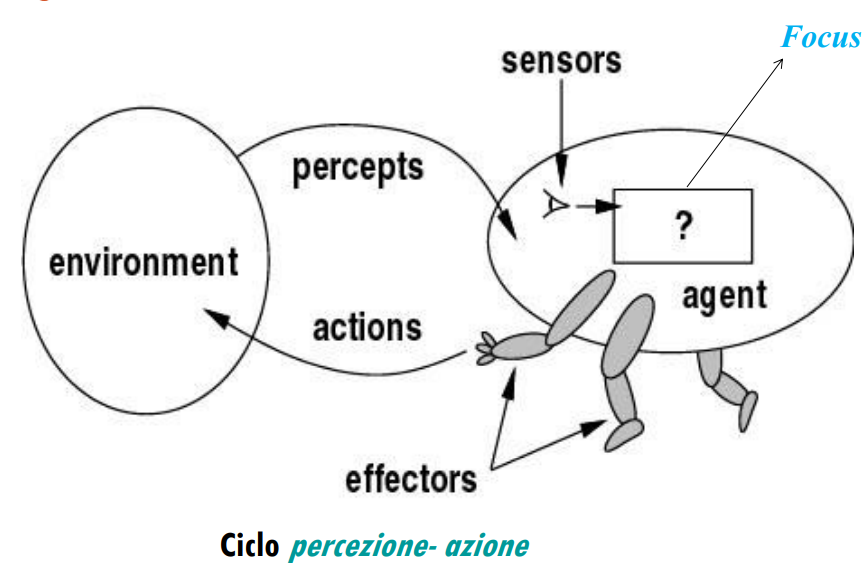
\includegraphics[scale=0.7]{agenti.png}
\end{center}
\subsection{Caratteristiche}
Sono qualcosa di più di un modulo software.
\paragraph{Situati} Gli agenti sono \textbf{situati in un ambiente} da cui \textbf{ricevono percezioni} e su cui \textbf{agiscono} mediante \textbf{azioni} (\textbf{attuatori}).
\paragraph{Sociali} Gli agenti hanno \textbf{abilità sociali}: comunicano, collaborano e si difendono da altri agenti.
\paragraph{Credenze, obiettivi, intenzioni\ldots}
\paragraph{Corpo} Gli agenti hanno un \textbf{corpo}, sono \textbf{embodied} fino a considerare i meccanismi delle emozioni.
\subsection{Percezioni e Azioni}
\paragraph{Percezione} Una percezione è un input da sensori.
\paragraph{Sequenza percettiva} Storia \textbf{completa} delle percezioni\\
La \textbf{scelta delle azioni} è \textbf{unicamente determinata dalla sequenza percettiva}.
\paragraph{Funzione Agente} Definisce l'azione da intraprendere per ogni sequenza percettiva e \textbf{descrive completamente l'agente}. Implementata da un \textbf{programma agente}.
\begin{center}
	\textbf{Sequenza Percettiva} $\longrightarrow^f$ \textbf{Azione}
\end{center}
Il compito dell'IA è progettare il programma agente.
\subsection{Agente e ambiente}
\paragraph{Architettura astratta}
\begin{center}
	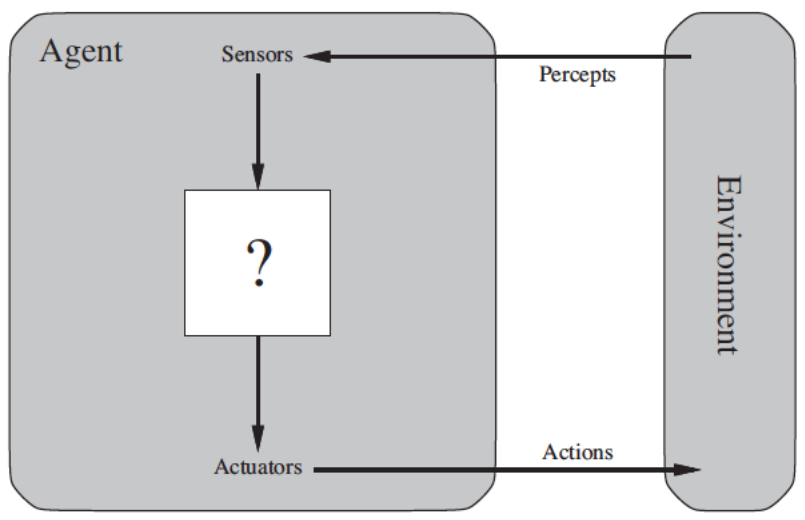
\includegraphics[scale=0.7]{ambiente.png}
\end{center}
\paragraph{Esempi}
\begin{list}{}{}
	\item \textbf{Agente robotico} Percepisce con camera, microfoni e sensori. Interagisce con motori, voce\ldots
	\item \textbf{Agente finanziario} Percepisce i tassi, le news. Interagisce con acquisti e scambi.
	\item \textbf{Agente di gioco} Percepisce le mosse dell'avversario. Interagisce tramite le proprie mosse.
	\item \textbf{Agente diagnostico} Percepisce i sintomi e le analisi dei pazienti. Interagisce fornendo la diagnosi.
	\item \textbf{Agente web} Percepisce le query utente e le pagine web. Interagisce fornendo i risultati di ricerca.
\end{list}
\subsection{Agenti Razionali}
\paragraph{Agenti razionali} Un agente razionale \textbf{interagisce con l'ambiente in maniera efficace}: "\textit{fa la cosa giusta}". L'agente razionale raggiunge l'obiettivo nella maniera più efficiente.\\
Serve quindi una \textbf{misura di prestazione}, di \textit{come vogliamo che il mondo evolva}, a seconda del problema e considerato l'ambiente.
\begin{list}{}{}
	\item \textbf{Esterna}, perché bisogna definirla \textit{prima} di agire. Non si può definire l'obiettivo dopo aver iniziato ad agire, altrimenti non è significativo.\\
	Esempio: la volpe che non arriva all'uva.
	\item Scelta dal progettista a seconda del problema e considerando l'effetto che ha sull'ambiente.
\end{list}
\paragraph{Razionalità} La razionalità è relativa/dipende da:
\begin{list}{}{}
	\item Misura delle prestazioni
	\item Conoscenze pregresse dell'ambiente
	\item Percezioni presenti e passate (sequenza percettiva)
	\item Capacità dell'agente (le azioni possibili)
\end{list}
\paragraph{Definizione} Un \textbf{agente razionale}, quindi, \textbf{esegue l'azione che massimizza il valore atteso della misura delle prestazioni per ogni sequenza di percezioni}, considerando le sue percezioni passate e la sua conoscenza pregressa.\\
Non si pretende perfezione e conoscenza del futuro, ma massimizzare il risultato \textit{atteso}. Potrebbero essere necessarie azioni di acquisizione di informazioni o esplorative (\textbf{non onniscenza}).\\
Le capacità dell'agente possono essere limitate (\textbf{non onnipotenza}).
\paragraph{Razionalità e apprendimento} Raramente il programmatore può fornire a priori tutta la conoscenza sull'ambiente. L'agente razionale, quindi, \textbf{deve essere in grado di modificare il proprio comportamento con l'esperienza}, cioè con le percezioni passate.\\
Può migliorarsi esplorando, \textbf{apprendendo}, aumentando la propria autonomia per operare in ambienti differenti o mutevoli.
\subsection{Agenti Autonomi} Un agente è \textbf{autonomo quando il suo comportamento dipende dalla sua esperienza}. Se il suo comportamento fosse determinato solo dalla propria conoscenza \textit{built-int} allora sarebbe \textbf{non autonomo} e poco flessibile.
\pagebreak
\section{Ambienti}
Definire un problema per un agente significa \textbf{caratterizzare l'ambiente in cui lavora}, cioè l'\textbf{ambiente operativo}. L'agente razionale è la soluzione del problema.
\subsection{PEAS}
\begin{list}{}{}
	\item \textbf{Performance}, prestazioni
	\item \textbf{Environment}, ambiente
	\item \textbf{Actuators}, attuatori
	\item \textbf{Sensors}, sensori
\end{list}
\paragraph{Esempio} Autista di taxi
\begin{center}
	\begin{tabular}{p{4cm} | p{4cm} | p{4cm} | p{4cm}}
		\textbf{Prestazione} & \textbf{Ambiente} & \textbf{Attuatori} & \textbf{Sensori} \\
		\hline
		Arrivare alla destinazione, sicuro, veloce, ligio alla legge, confortevole, consumo minimo di benzina, profitti massimi & Strada, altri veicoli, clienti & Sterzo, acceleratore, freni, frecce, clacson & Telecamere, sensori, GPS, contachilometri, accelerometro, sensori del motore\ldots
	\end{tabular}
\end{center}
\paragraph{Formulazione PEAS dei problemi}
\begin{center}
	\begin{tabular}{p{3cm} | p{3cm} | p{3cm} | p{3cm} | p{3cm}}
		\textbf{Problema} & \textbf{P} & \textbf{E} & \textbf{A} & \textbf{S} \\
		\hline
		Diagnosi medica & Diagnosi corretta & Pazienti, ospedale & Domande, suggerimenti, test, diagnosi & Sintomi, test clinici, risposte del paziente \\
		\hline
		Analisi immagini & Numero di immagini/zone correttamente classificate & Collezione di fotografie & Etichettatore di zone nell'immagine & Array di pixel \\
		\hline
		Robot "selezionatore" & Numero delle parti correttamente classificate & Nastro trasportatore & Raccogliere le parti e metterle nei cestini & Telecamera (pixel di varia intensità) \\
		\hline
		Giocatore di calcio & Fare più goal dell'avversario & Altri giocatore, campo di calcio, porte & Dare calci al pallone, correre & Locazione del pallone, dei giocatori e delle porte
	\end{tabular}
\end{center}
\subsection{Simulatore di Ambienti}
Uno \textbf{strumento software} con il compito di:
\begin{list}{}{}
	\item Generare gli stimoli per gli agenti
	\item Raccogliere le azioni in risposta
	\item Aggiornare lo stato dell'ambiente
	\item Opzionalmente, attivare altri processi che influenzano l'ambiente
	\item Valutare le prestazioni degli agenti
\end{list}
Gli esperimenti su classi di ambienti (variando le condizioni) sono essenziali per valutare la capacità di generalizzare. La valutazione delle prestazioni è fatta tramite la media su più istanze.
\pagebreak
\subsection{Proprietà dell'Ambiente-Problema}
\begin{list}{-}{}
	\item \textbf{Osservabilità}\\\textbf{Completamente osservabile}: l'apparato percettivo è in grado di dare una conoscenza completa dell'ambiente o almeno tutto quello che serve a decidere l'azione.\\
	\textbf{Parzialmente osservabile}: sono presenti limiti o inaccuratezze nell'apparato sensoriale. (Es. la videocamera di un rover vede solo parte dell'ambiente in un dato istante).
	\item \textbf{Singolo/Multi-Agente}\\
	Distinzione tra agente e non agente: il mondo può cambiare anche attraverso \textbf{eventi}, non necessariamente per le azioni di agenti.\\
	\textbf{Multi-Agente Competitivo}, come gli scacchi: comportamento randomizzato ma razionale.\\
	\textbf{Multi-Agente Cooperativo}, o benigno: stesso obiettivo e comunicazione.
	\item \textbf{Predicibilità}\\
	\textbf{Deterministico}: lo stato successivo è completamente determinato dallo stato corrente e dall'azione.\\
	\textbf{Stocastico}: esistono elementi di incertezza con probabilità associata. Es: guida, tiro in porta.\\
	\textbf{Non deterministico}: si tiene traccia di più stati possibili che sono risultato dell'azione, ma non in base ad una probabilità.
	\item \textbf{Episodico}: l'esperienza dell'agente è divisa in episodi atomici indipendenti. In ambienti episodici non c'è bisogno di pianificare.\\
	\textbf{Sequenziale}: ogni decisione influenza le succesive.
	\item \textbf{Statico}: il mondo non cambia mentre l'agente decide l'azione.\\
	\textbf{Dinamico}: l'ambiente cambia nel tempo, va osservata la contingenza. Tardare equivale a non agire.\\
	\textbf{Semi-dinamico}: l'ambiente non cambia ma la valutazione dell'agente si. Es: scacchi con timer, se non agisco prima dello scadere perdo.
	\item \textbf{Discreto/Continuo}\\
	Lo stato, il tempo, le percezioni e le azioni sono tutti elementi che possono assumere valori discreti o continui.\\
	Combinatoriale (nel discreto) \textit{vs} infinito (nel continuo).
	\item \textbf{Noto/Ignoto}\\
	Distinzione riferita allo stato di conoscenza dell'agente sulle leggi fisiche dell'ambiente. L'\textbf{agente conosce l'ambiente o deve compiere azioni esplorative}?\\
	\textbf{Noto $\neq$ osservabile}: posso giocare a carte coperte, ma con regole note.
\end{list}
\paragraph{Ambienti reali} Parzialmente osservabili, stocastici, sequenziali, dinamici, continui, multi-agente e ignoti.
\pagebreak

\section{Struttura di un Agente}
\begin{center}
\textbf{Agente $=$ Architettura $+$ Programma}\\
Ag: P $\longrightarrow$ Az
\end{center}
L'\textbf{Ag}ente associa \textbf{Az}ioni alle \textbf{P}ercezioni. Il \textbf{programma dell'agente} implementa la funzione \textbf{Ag}.
\paragraph{Programma Agente} Pseudocodice del programma agente.
\begin{center}
\begin{lstlisting}
function Skeleton-Agent(percept) returns action
	static: memory #la memoria del mondo posseduta dall'agente
	memory <- UpdateMemory(memory, percept)
	action <- Choose-Best-Action(memory) #Cuore dell'IA
	memory <- UpdateMemory(memory, action)
	return action
\end{lstlisting}
\end{center}
\subsection{Strutture di Agenti Caratteristici}
\paragraph{Agente basato su tabella} La scelta dell'azione è un accesso ad una tabella che \textbf{associa un'azione ad ogni possibile sequenza di percezioni}.\\
Vari \textbf{problemi}:
\begin{list}{}{}
	\item Le \textbf{dimensioni} possono essere proibitive: per giocare a scacchi, la tabella dovrebbe contenere un numero di righe nell'ordine di $10^{120} >> 10^{80}$ numero di atomi nell'universo osservabile.
	\item \textbf{Difficile da costruire}
	\item \textbf{Nessuna autonomia}
	\item \textbf{Difficile da aggiornare}, apprendimento complesso.
\end{list}
Con le IA vogliamo realizzare \textbf{automi razionali con un programma \textit{compatto}}.

\paragraph{Agente Reattivo Semplice}
\begin{center}
	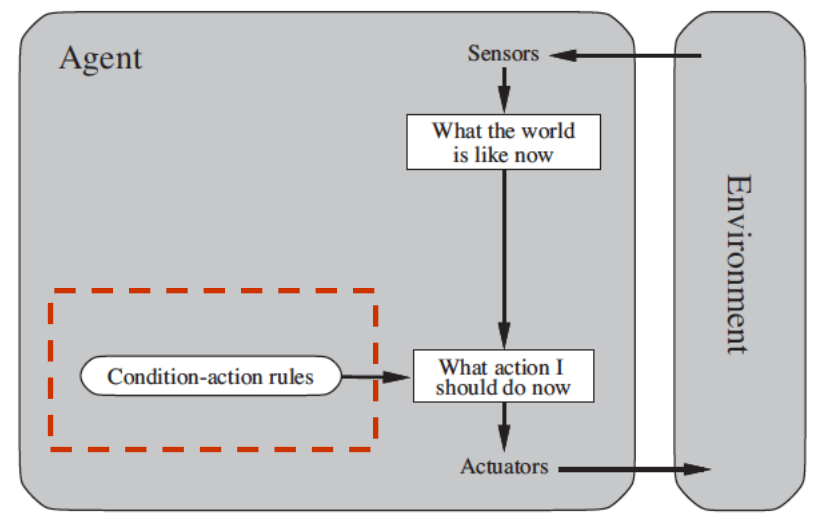
\includegraphics[scale=0.5]{agreattsemplice.png}
\end{center}
\begin{lstlisting}
function Agente-Reattivo-Semplice(percezione) returns azione
	persistent: regole #insieme di regole condizione-azione (if-then)
	stato <- Interpreta-Input(percezione)
	regola <- Regola-Corrispondente(stato, regole)
	azione <- regola.Azione
	return azione
\end{lstlisting}
\paragraph{Agenti basati su modello}
\begin{center}
	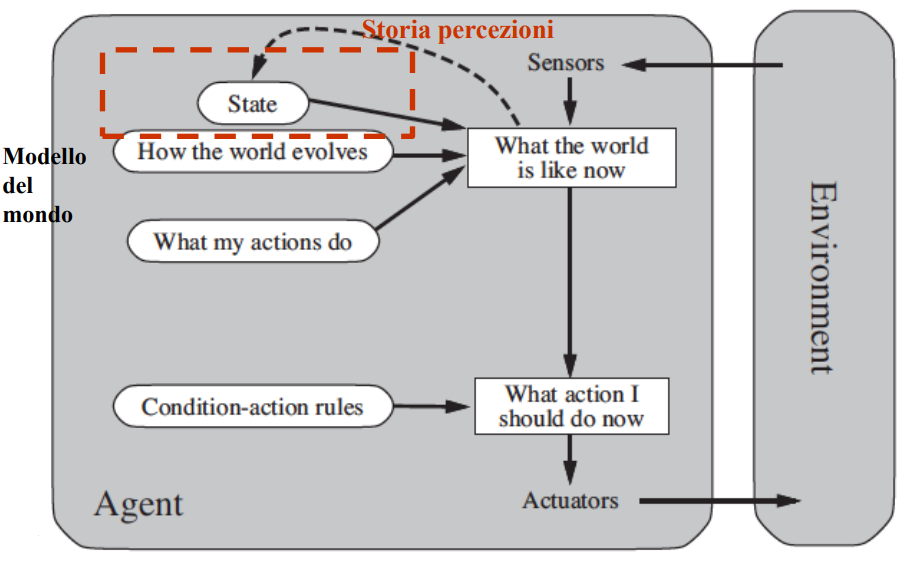
\includegraphics[scale=0.5]{agmodello.png}
\end{center}
\begin{lstlisting}
function Agente-Basato-su-Modello(percezione) returns azione
	persistent:	stato #descrizione dello stato corrente
			modello #conoscenza del mondo
			regole #insieme di regole condizione-azione
			azione #azione piu recente
	stato <- Aggiorna-Stato(stato, azione, percezione, modello)
	regola <- Regola-Corrispondente(stato, regole)
	azione <- regola.Azione
	return azione
\end{lstlisting}
\paragraph{Agenti con obiettivo} Bisogna pianificare una sequenza di azioni per raggiungere l'obiettivo. (In rosso sono indicate le parti aggiunte)
\begin{center}
	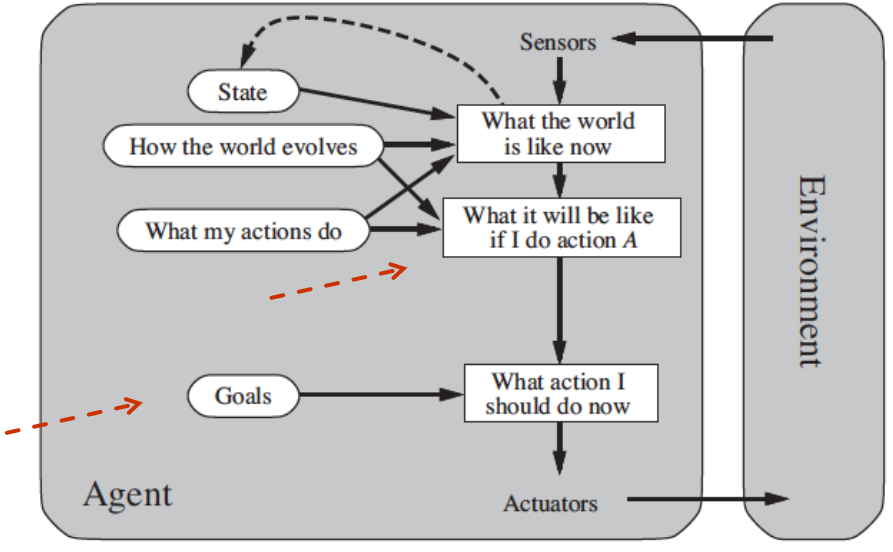
\includegraphics[scale=0.5]{agobiettivo.png}
\end{center}
Sono \textbf{guidati da un obiettivo nella scelta che intraprendono}, è stato fornito un \textbf{goal esplicito}: per esempio una città da raggiungere.\\
A volte l'azione migliore dipende dall'obiettivo da raggiungere (\textit{da che parte devo girare?})\\
Devo \textbf{pianificare una sequenza di azioni} per raggiungere l'obiettivo. Sono meno efficienti ma \textbf{più flessibili} rispetto ad un agente reattivo. L'obiettivo può cambiare, non è codificato nelle regole.\\
Esempio classico: ricerca della sequenza di azioni per raggiungere una data destinazione.
\paragraph{Agenti con valutazione di utilità}
\begin{center}
	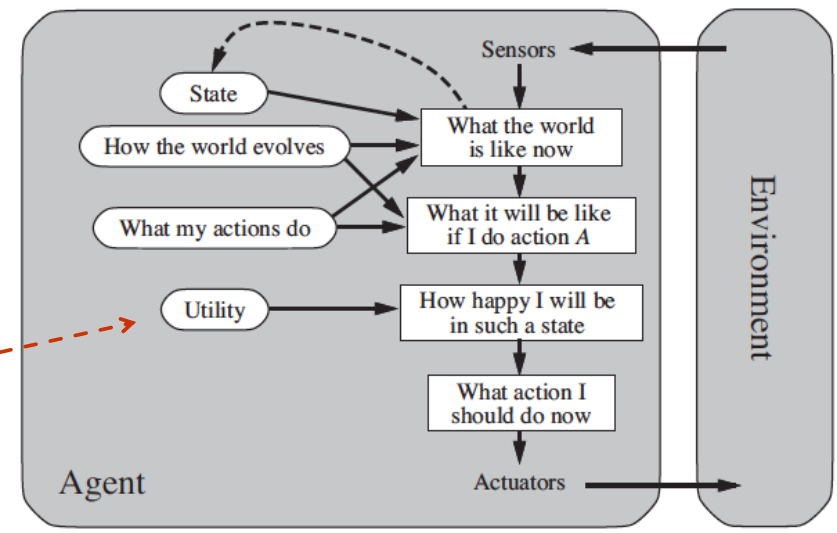
\includegraphics[scale=0.5]{agvalutazutilita.png}
\end{center}
\textbf{Obiettivi alternativi}, o più modi per raggiungerlo: l'agente deve decidere verso quali muoversi, quindi è \textbf{necessaria una funzione di utilità} che associa ad uno stato obiettivo un numero reale.\\
\textbf{Obiettivi più facilmente raggiungibili di altri}: la funzione di utilità \textbf{tiene conto della probabilità di successo} e/o di ciascun risultato (\textbf{utilità attesa} o media)
\paragraph{Agenti che apprendono}
\begin{center}
	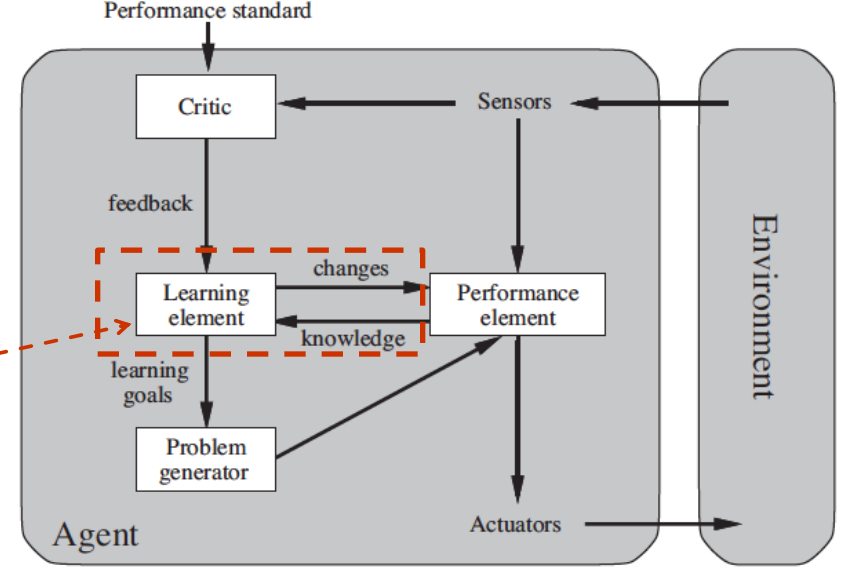
\includegraphics[scale=0.5]{agappr.png}
\end{center}
\begin{list}{}{}
	\item \textbf{Componente di apprendimento}: produce cambiamenti al programma agente. Migliora le prestazioni, adattando i suoi componenti ed apprendendo dall'ambiente
	\item \textbf{Elemento esecutivo}: il programma agente
	\item \textbf{Elemento critico}: osserva e dà feedback sul comportamento
	\item \textbf{Generatore di problemi}: suggerisce nuove situazioni da esplorare
\end{list}
\pagebreak
\subsection{Tipi di rappresentazione}
\paragraph{Stati e transizioni}
\begin{center}
	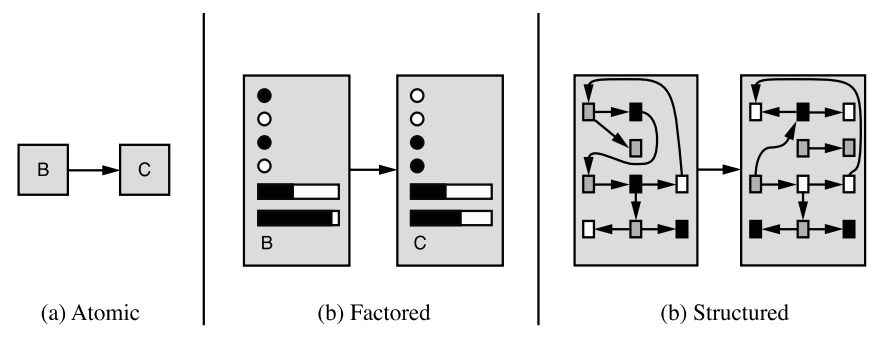
\includegraphics[scale=0.75]{rapprstatitransizioni.png}
\end{center}
\begin{list}{}{}
	\item \textbf{Rappresentazione atomica} (stati)
	\item \textbf{Rappresntazione fattorizzata} ($+$ variabili e attributi)
	\item \textbf{Rappresentazione strutturata} ($+$ relazioni)
\end{list}

\chapter{Problem Solving}
\section{Agenti Risolutori di Problemi}
\paragraph{Problem Solving} Questi agenti adottano il paradigma della \textbf{risoluzione di problemi come ricerca in uno spazio di stati} (\textbf{problemi solving}). Sono \textbf{agenti con modello} (storia, percezioni) che \textbf{adottano una rappresentazione atomica dello stato}. Sono \textbf{particolari agenti con obiettivo} che \textbf{pianificano l'intera sequenza di azioni} prima di agire.
\subsection{Processo di risoluzione}
\paragraph{Passi da seguire}
\begin{enumerate}
	\item \textbf{Determinazioni dell'obiettivo}: un insieme di stati dove l'obiettivo è soddisfatto.
	\item \textbf{Formulazione del problema}: rappresentazione degli stati e delle azioni.\\
	\textit{Fa parte del design "umano"}.
	\item \textbf{Determinazione della soluzione} mediante ricerca: un piano d'azione
	\item \textbf{Esecuzione del piano}\\
	\textit{Soluzione algoritmica}.
\end{enumerate}
La determinazione dell'obiettivo e la formulazione del problema richiede \textbf{tanta intelligenza}, che in fase di design è \textbf{spostata sull'umano}. Gli algoritmi sono ancora "\textit{stupidi}".
\paragraph{Assunzioni sull'ambiente} \textbf{Statico}, \textbf{osservabile} (so dove sono, es: \textit{viaggio con la mappa}), \textbf{discreto} (insieme finito di azioni possibili), \textbf{deterministico} (una azione $\Rightarrow$ un risultato. L'agente può eseguire il piano "\textit{ad occhi chiusi}", niente può andare storto)
\paragraph{Formulazione del problema} Un problema può essere \textbf{definito formalmente} mediante cinque componenti:
\begin{enumerate}
	\item \textbf{Stato iniziale}
	\item \textbf{Azioni possibili} nello stato \texttt{s}: \texttt{Azioni(s)}
	\item \textbf{Modello di transizione}\\
	\texttt{Risultato}: stato $\times$ azione $\longrightarrow$ stato\\
	\texttt{Risultato(s, a)}: \texttt{s'}, uno stato \textbf{successore}
	\item \textbf{Test obiettivo}: un insieme di stati obiettivo\\
	\texttt{Goal-Test}: stato $\longrightarrow$ \{\texttt{true}, \texttt{false}\}
	\item \textbf{Costo del cammino}: somma dei costi delle azioni (costo dei passi).\\
	Costo di un passo: \texttt{c(s, a, s')}, mai negativo.
\end{enumerate}
1, 2 e 3 \textbf{definiscono \textit{implicitamente} lo spazio degli stati}. Definirlo esplicitamente può essere molto oneroso, come in quasi tutti i problemi di IA.
\pagebreak
\section{Algoritmi di Ricerca}
\textit{Il processo che cerca una sequenza di azioni che raggiunge l'obiettivo è detto \textbf{ricerca}}.
\paragraph{Algoritmi} Gli algoritmi di ricerca prendono in \textbf{input un problema} e \textbf{restituiscono un cammino soluzione}, un cammino che porta dallo stato iniziale allo stato goal.
\paragraph{Misura delle prestazioni} Trova una soluzione? Quanto costa trovarla? Quanto è efficiente la soluzione?
\begin{center}
Costo Totale = Costo della Ricerca $+$ Costo del Cammino Soluzione
\end{center}
Valuteremo algoritmi sul primo, ottimizzando il secondo.
\subsection{Ricerca ad Albero}
Generazione di un \textbf{albero di ricerca sovrapposto allo spazio degli stati}. Ricerca significa \textbf{approfondire l'opzione}, mettendo da parte le altre che verranno riprese se non trovo la soluzione.\\
Quindi l'albero viene generato esplorando i vari nodi partendo dallo stato iniziale. Il nodo è diverso dallo stato: per esempio, in un grafo rappresentante le città, se parto da città A ed esploro l'opzione nodo B, il nodo B avrà come figlio anche città A perché posso tornarci.
\begin{center}
	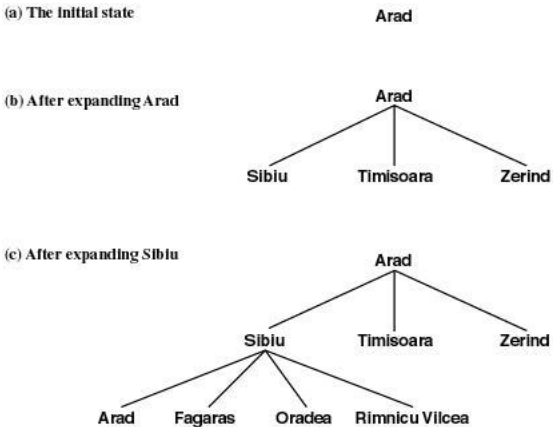
\includegraphics[scale=0.7]{ricercaalbero.png}
\end{center}
\paragraph{Algoritmo} \textbf{Ricerca ad albero}, ossia senza controllare se i nodi (\textbf{stati}) siano già stati esplorati.

\begin{lstlisting}
function Ricerca-Albero(problema) returns soluzione oppure fallimento
	#Inizializza la frontiera con stato iniziale del problema
	loop do
	if (frontiera vuota) 
		return fallimento
	#Scegli* un nodo foglia da espandere e rimuovilo dalla frontiera
	if (nodo contiene uno stato obiettivo)
		return soluzione corrispondente
	#Espandi il nodo e aggiungi i successori alla frontiera
\end{lstlisting}
$*$ $=$ \textbf{strategia}: quale scegliere? I vari algoritmi si differenziano per la strategia di scelta.\\
\begin{list}{}{Un \textbf{nodo} n è una \textbf{struttura dati con quattro componenti}}
	\item \textbf{Stato}, n.stato
	\item \textbf{Padre}, n.padre
	\item \textbf{Azione} effettuata per generarlo, n.azione
	\item \textbf{Costo} del cammino dal nodo iniziale al nodo, n.costo-cammino\\
	Indicata come g(b) = padre.costo-cammino + costo-passo ultimo)
\end{list}
\paragraph{Frontiera} Lista dei \textbf{nodi in attesa di essere espansi}, cioè \textbf{le foglie} dell'albero di ricerca. Implementata come una coda con operazioni:
\begin{list}{}{}
	\item Vuota(coda)
	\item Pop(coda) estrae l'ultimo elemento (implementa la strategia)
	\item Inserisci(elemento, coda)
\end{list}
Diversi tipi di coda hanno differenti funzioni di inserimento e \textbf{implementano strategie diverse}.
\begin{list}{}{}
	\item \textbf{FIFO} $\rightarrow$ BF\\
	Viene estratto l'elemento più vecchio, cioè in attesa da più tempo. Nuovi nodi aggiunti alla fine
	\item \textbf{LIFO} $\rightarrow$ DF\\
	Viene estratto l'ultimo elemento inserito. Nuovi nodi aggiunti all'inizio
	\item \textbf{Con priorità} $\rightarrow$ UC, altri\ldots\\
	Viene estratto l'elemento con priorità più alta in base ad una funzione di ordinamento. All'aggiunta di un nuovo nodo si riordina.
\end{list}
\paragraph{Strategie non informate}
\begin{list}{}{}
	\item Ricerca in \textbf{ampiezza} (BF)
	\item Ricerca in \textbf{profondità} (DF)
	\item Ricerca in \textbf{profondità limitata} (DL)
	\item Ricerca con \textbf{apprendimento iterativo} (ID)
	\item Ricerca di \textbf{costo uniforme} (UC)
\end{list}
\paragraph{Strategie informate} Anche dette di \textbf{ricerca euristica}: fanno uso di informazioni riguardo la distanza stimata della soluzione.
\paragraph{Valutazione di una strategia}
\begin{list}{}{}
	\item \textbf{Completezza}: se la soluzione esiste viene trovata
	\item \textbf{Ottimalità} (ammissibilità): trova la soluzione migliore, con costo minore
	\item \textbf{Complessità in tempo}: tempo richiesto per trovare la soluzione
	\item \textbf{Complessità in spazio}: memoria richiesta
\end{list}
\subsection{Breadth-First}
\paragraph{Ricerca in ampiezza} Esplorare il grafo dello spazio degli stati a livelli progressivi di stessa profondità. Implementata con una coda FIFO. \textbf{Algoritmo su albero}:
\begin{lstlisting}
function RicercaAmpiezzaA(problema)	returns soluzione oppure fallimento
	nodo = un nodo con stato = problema.stato-iniziale e costo-di-cammino = 0
	#Stati goal-tested alla generazione: maggior efficienza si ferma appena trova goal
	if (problema.TestObiettivo(nodo.Stato)) return Soluzione(nodo)
	frontiera = una coda FIFO con nodo come unico elemento
	loop do
	if (Vuota(frontiera)) return fallimento
	nodo = Pop(frontiera)
	for each azione in problema.Azioni(nodo.Stato) do #Espansione
		figlio = Nodo-Figlio(problema, nodo, azione) #costruttore: vedi AIMA
		if (Problema.TestObiettivo(figlio.Stato)) return Soluzione(figlio)
		frontiera = Inserisci(figlio, frontiera) #frontiera coda FIFO
\end{lstlisting}
\pagebreak
\textbf{Algoritmo su grafo} evitando di espandere stati già esplorati:
\begin{lstlisting}
function RicercaAmpiezzaG(problema) returns soluzione oppure fallimento
	nodo = un nodo con stato = problema.stato-iniziale e costo-di-cammino = 0
	if (problema.TestObiettivo(nodo.Stato)) return Soluzione(nodo)
	frontiera = una coda FIFO con nodo come unico elemento
	esplorati = insieme vuoto #gestisco stati ripetuti
	loop do
	if (Vuota(frontiera)) return fallimento
	nodo = POP(frontiera) #aggiungi nodo.Stato a esplorati
	for each azione in problema.Azioni(nodo.Stato) do
		figlio = Nodo-Figlio(problema, nodo, azione)
		if (figlio.Stato non in esplorati e non in frontiera)
			if (Problema.TestObiettivo(figlio.Stato)) return Soluzione(figlio)
			frontiera = Inserisci(figlio, frontiera) #in coda
\end{lstlisting}

\textbf{Python}
\begin{lstlisting}
def breadth_first_search(problem): """Ricerca-grafo in ampiezza"""
  explored = [] # insieme degli stati gia' visitati (implementato come una lista)
  node = Node(problem.initial_state) #il costo del cammino e' inizializzato nel costruttore del nodo
  if problem.goal_test(node.state):
    return node.solution(explored_set = explored)
  frontier = FIFOQueue() # la frontiera e' una coda FIFO
  frontier.insert(node)
  while not frontier.isempty(): # seleziona il nodo per l'espansione
    node = frontier.pop()
    explored.append(node.state) # inserisce il nodo nell'insieme dei nodi esplorati
    for action in problem.actions(node.state):
      child_node = node.child_node(problem,action)
      if (child_node.state not in explored) and
      (not frontier.contains_state(child_node.state)):
        if problem.goal_test(child_node.state):
        return child_node.solution(explored_set = explored)
      # se lo stato non e' uno stato obiettivo allora inserisci il nodo nella frontiera
      frontier.insert(child_node)
  return None # in questo caso ritorna con fallimento
\end{lstlisting}
\paragraph{Analisi della complessità spazio-temporale} Assumiamo:
\begin{list}{}{}
	\item \textbf{b} = fattore di ramificazione (\textbf{b}ranching)
	\item \textbf{d} = profondità del nodo obiettivo più superficiale (\textbf{d}epth)\\
	Più vicino all'iniziale
	\item \textbf{m} = lunghezza massima dei cammini nello spazio degli stati (\textbf{m}ax)
\end{list}
Analisi:
\begin{list}{}{}
	\item Strategia \textbf{completa}
	\item Strategia \textbf{ottimale} \textit{se gli operatori hanno tutti lo stesso costo k} cioè g(n) = k $\cdot$ depth(n), dove g(n) è il costo del cammino per arrivare ad n.
	\item Complessità nel tempo (nodi generati)\\
	T(b, d) = b + b$^2$ + \ldots + b$^d$ = O(b$^d$), con b figli per ogni nodo.
	\item Complessità nello spazio (nodi in memoria): O(b$^d$)
\end{list}
\pagebreak
\subsection{Depth-First}
\paragraph{Ricerca in profondità} Implementata da una coda che mette i successori in testa alla lista (LIFO, pila o stack). Algoritmo generale visto all'inizio, su grafo o albero.
\paragraph{Analisi (su albero)} Poniamo \textbf{m} lunghezza massima dei cammini nello spazio degli stati e \textbf{b} fattore di diramazione\\
Tempo: O(b$^m$) che può essere anche $>$ O(b$^d$)\\
Spazio: b$\cdot$m, frontiera sul cammino perché vengono cancellati i rami completamente esplorati ma mantenuti i fratelli del path corrente.\\
\textbf{Non completa} (loop) e \textbf{non ottimale}, ma drastico risparmio di memoria.
\begin{list}{}{}
	\item BF, d = 16 $\rightarrow$ 10 Esabyte
	\item DF, d = 16 $\rightarrow$ 156 Kilobyte
\end{list}
\paragraph{Analisi (su grafo)} In caso di DF su grafo si perdono i vantaggi di memoria: torna a tutti i possibili stati (al caso pessimo diventa esponenziale come BF) per mantenere la lista dei visitati, ma così DF diventa \textbf{completa} in spazi degli stati finiti (al caso pessimo tutti i nodi vengono espansi).\\
Rimane non completa in spazi infiniti.\\
Possibile controllare anche solo i nuovi stati rispetto al cammino radice-nodo corrente senza aggravio di memoria. Si evitano i cicli finiti in spazi finiti ma non i cammini ridondanti.
\subsection{Depth-First ricorsiva}
Ancora più efficiente in occupazione di memoria perché mantiene solo il cammino corrente (m nodi al caso pessimo).\\
Realizzata da un algoritmo ricorsivo "con backtracking" che non necessita di tenere in memoria b nodi per ogni livello, ma salva lo stato su uno stack a cui torna in caso di fallimento per fare altri tentativi. \textbf{Algoritmo su albero}:
\begin{lstlisting}
function Ricerca-DF-A (problema) returns soluzione oppure fallimento
	return Ricerca-DF-ricorsiva(CreaNodo(problema.Stato-iniziale), problema)
	
function Ricerca-DF-ricorsiva(nodo, problema) returns soluzione oppure fallimento
	if problema.TestObiettivo(nodo.Stato) return Soluzione(nodo)
	else
		for each azione in problema.Azioni(nodo.Stato) do
			figlio = Nodo-Figlio(problema, nodo, azione)
			risultato = Ricerca-DF-ricorsiva(figlio, problema)
			if risultato != fallimento then return risultato
		return fallimento
\end{lstlisting}
\textbf{Python}
\begin{lstlisting}
def recursive_depth_first_search(problem, node):  """Ricerca in profondita' ricorsiva """
  #controlla se lo stato del nodo e' uno stato obiettivo
   if problem.goal_test(node.state):
    return node.solution()
  #in caso contrario continua
  for action in problem.actions(node.state):
    child_node = node.child_node(problem, action)
    result = recursive_depth_first_search(problem, child_node)
    if result is not None: return result
  return None #con fallimento
\end{lstlisting}
\subsection{Depth-Limited}
\paragraph{Ricerca in profondità limitata} Si va in profondità fino ad un certo livello predefinito \textbf{l}.\\
\textbf{Completa} per poblemi di cui si conosce un limite superiore per la profondità della soluzione: ad esempio route-finding limitata dal numero di città - 1\\
\textbf{Completo} se d $<$ l\\
\textbf{Non ottimale}\\
Complessità in tempo: O(b$^l$)\\
Complessità in spazio: O(b$\cdot$l)
\pagebreak
\subsection{Iterative-Deepening}
\begin{center}
	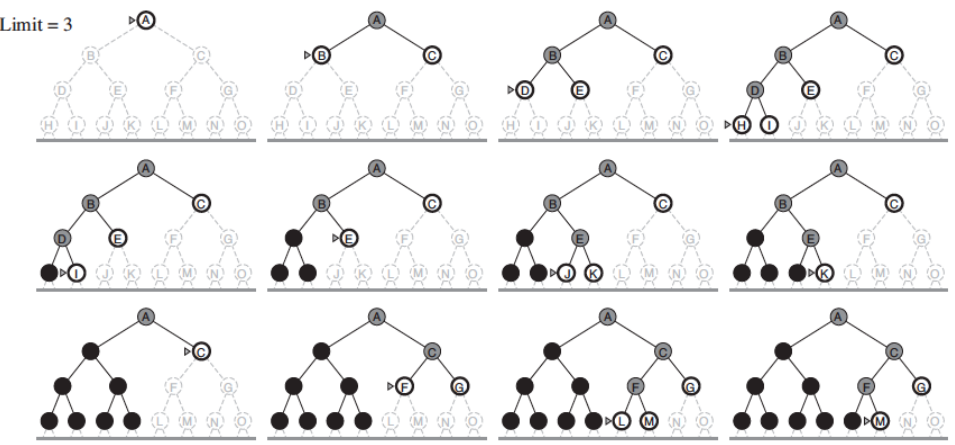
\includegraphics[scale=0.7]{id.png}
\end{center}
\paragraph{Analisi} Miglior compromesso tra BF e DF. Nell'ID, i nodi dell'ultimo livello sono generati una volta, quelli del penultimo 2, del terzultimo 3\ldots quelli del primo d volte.\\ID: (d)b + (d-1)b$^2$ + \ldots + 3b$^{d-2}$ + 2b$^{d-1}$ + b$^d$\\
Complessità in tempo: O(b$^d$)\\
Complessità in spazio: O(b$\cdot$d), vs O(b$^d$) del BF.
\section{Direzione della Ricerca}
Altro aspetto usato per ottimizzare la risoluzione di problemi, la \textbf{direzione della ricerca} è un \textbf{problema ortogonale alla strategia di ricerca}. La ricerca si può fare
\begin{list}{}{}
	\item \textbf{In avanti}, guidata dai dati come fatto fin'ora: si \textbf{esplora lo spazio di ricerca dallo stato iniziale allo stato obiettivo}
	\item \textbf{All'indietro} o \textbf{guidata dall'obiettivo}: si \textbf{esplora lo spazio di ricerca a partire da un goal e riconducendosi a sotto-goal fino a trovare uno stato iniziale}.
\end{list}
Conviene \textbf{procedere nella direzione in cui il fattore di diramazione è minore}.\\
Si preferisce la \textbf{ricerca all'indietro} quando
\begin{list}{}{}
	\item l'\textbf{obiettivo è chiaramente definito} (es. theorem proving) o si possono \textbf{formulare una serie limitata di ipotesi}
	\item i \textbf{dati del problema non sono noti} e la loro \textbf{acquisizione può essere guidata dall'obiettivo}
\end{list}
mentre si preferisce la \textbf{ricerca in avanti} quando
\begin{list}{}{}
	\item gli \textbf{obiettivi possibili sono molti} (es. design)
	\item abbiamo una \textbf{serie di dati da cui partire}
\end{list}
\pagebreak
\paragraph{Ricerca bidirezionale} Si procede nelle due direzioni fino ad incontrarsi
\begin{multicols}{2}
\begin{list}{}{}
	\item \textbf{Complessità in tempo}: O(b$^{d/2}$) = O($\sqrt{b^d}$)\\Test intersezione in tempo costante, esempio: hash table
	\item \textbf{Complessità in spazio}: O(b$^{d/2}$) = O($\sqrt{b^d}$)\\Almeno tutti i nodi in una direzione in memoria, esempio: usando BF
\end{list}
Non è sempre applicabile, ad esempio in casi di predecessori non definiti, troppi stati obiettivo\ldots
\begin{center}
	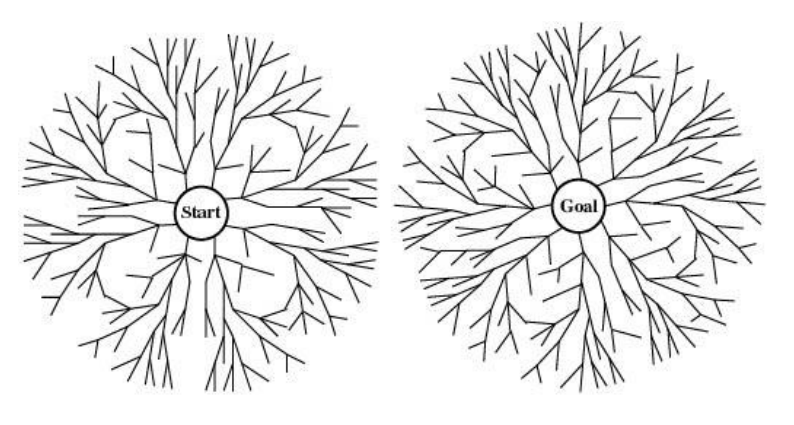
\includegraphics[scale=0.5]{ricbidirez.png}
\end{center}
\end{multicols}
\section{Problematiche}
\paragraph{Cammini Ciclici}
I \textbf{cammini ciclici} potenzialmente rendono gli alberi di ricerca infiniti, anche se con stati finiti.
\begin{center}
	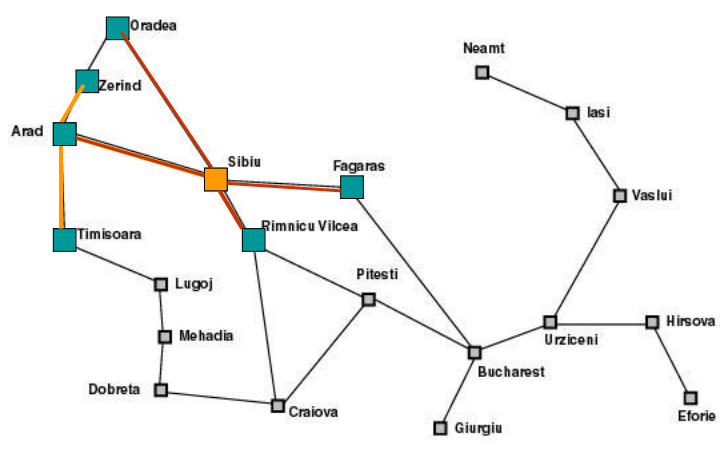
\includegraphics[scale=0.7]{camminiciclici.png}
\end{center}
\paragraph{Ridondanze}
Su spazi di stati a grafo si generano più volte nodi con lo stesso stato nella ricerca, anche in assenza di cicli.
\begin{center}
	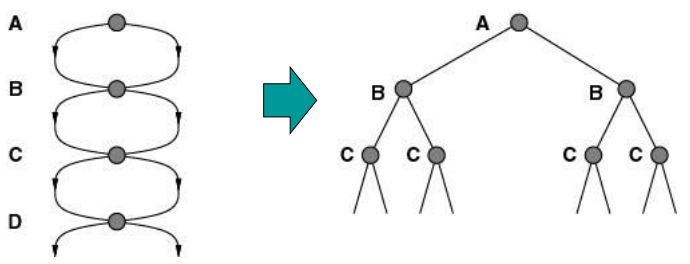
\includegraphics[scale=0.7]{ridondanze.png}
\end{center}
\pagebreak
Un caso è la \textbf{ricerca nelle griglie} Visitare stati già visitati fa compiere lavoro inutile. Costo 4$^d$ ma circa 2d$^2$ stati distinti.
\begin{center}
	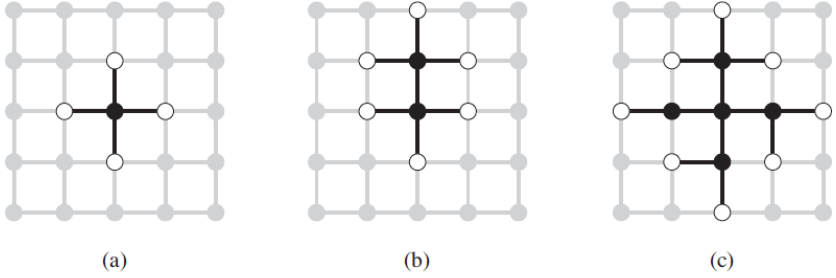
\includegraphics[scale=0.7]{griglie.png}
\end{center}
\textbf{Come evitarlo?}
\paragraph{Compromesso tra spazio e tempo} \textbf{Ricordare} gli stati visitati \textbf{occupa spazio} ma ci \textbf{consente di evitare di visitarli di nuovo}. \textit{Gli algoritmi che dimenticano la propria storia sono destinati a ripeterla}.
\subsection{Tre soluzioni} In ordine crescente di costo ed efficacia:
\begin{list}{}{}
	\item Non tornare nello stato da cui si proviene: si elimina il genitore dai nodi successori.\\
	Non evita i cammini ridondanti.
	\item Non creare cammini con cicli: si controlla che i successori non siano antenati del nodo corrente.
	\item Non generare nodi con stati già visitati/esplorati: ogni nodo visitato deve essere tenuto in memoria per una complessità O(s) dove s è il numero di stati possibili (esempio: hash table per accesso efficiente
\end{list}
\paragraph{Repetita} Il costo può essere alto: in caso di DF la memoria torna da b$\cdot$m a tutti gli stati, ma diventa una ricerca \textbf{completa} per spazi finiti. Ma \textbf{in molti casi gli stati crescono esponenzialmente} (scacchi\ldots)
\section{Uniform-Cost} \textbf{Generalizzazione della ricerca in ampiezza} (costi diversi tra passi): \textbf{si sceglie il nodo di costo g(n) del cammino minore sulla frontiera}, si espande sui contorni di uguale costo (e.g. in km) invece che sui contorni di uguale profondità (BF). Implementata da una \textbf{coda ordinata per costo cammino crescente}. \textbf{Algoritmo su albero}:
\begin{lstlisting}
function Ricerca-UC-A(problema) returns soluzione oppure fallimento
	nodo = un nodo con stato il problema.stato-iniziale e costo-di-cammino=0
	frontiera = una coda con priorita con nodo come unico elemento
	loop do
		if Vuota?(frontiera) then return fallimento
		nodo = POP(frontiera)
		#Esame post-generaz e vedere costo minore, tipico per coda con priorita
		if problema.TestObiettivo(nodo.Stato) then return Soluzione(nodo)
		for each azione in problema.Azioni(nodo.Stato) do
			figlio = Nodo-Figlio(problema, nodo, azione)
			frontiera = Inserisci(figlio, frontiera) #in coda con priorita
	end
\end{lstlisting}
\pagebreak
\textbf{Algoritmo su grafo}:
\begin{lstlisting}
function Ricerca-UC-G(problema) returns soluzione oppure fallimento
	nodo = un nodo con stato il problema.stato-iniziale e costo-di-cammino=0
	frontiera = una coda con priorita con nodo come unico elemento
	esplorati = insieme vuoto
	loop do
		if Vuota?(frontiera) then return fallimento
		nodo = POP(frontiera);
		if problema.TestObiettivo(nodo.Stato) then return Soluzione(nodo)
		aggiungi nodo.Stato a esplorati
		for each azione in problema.Azioni(nodo.Stato) do
			figlio = Nodo-Figlio(problema, nodo, azione)
			if figlio.Stato non in esplorati e non in frontiera then
				frontiera = Inserisci(figlio, frontiera) #in coda con priorita
			else if figlio.Stato in frontiera con Costo-cammino piu alto then
				sostituisci quel nodo frontiera con figlio 
\end{lstlisting}
\paragraph{Analisi} Ottimalità e completezza garantite purché il costo degli archi sia maggiore di $\epsilon > 0$. Assunto C$^*$ come il costo della soluzione ottima, allora $\lfloor$C$^*$/$\epsilon\rfloor$ \textbf{numero di mosse al caso peggiore}, arrotondato per difetto. Tendo ad andare verso tante mosse di costo $\epsilon$ prima di una che parta più alta ma poi abbia un path a costo più basso.\\
Complessità: O(b$^{1 + \lfloor C^*/\epsilon\rfloor}$).\\
Quando ogni azione ha lo stesso costo somiglia a BF ma con complessità O(b$^{1 + d}$) perché esame e arresto solo dopo aver espanso anche l'ultima frontiera.
\section{Confronto delle Strategie (albero)}
\begin{center}
\begin{tabular}{c | c | c | c | c | c | c}
Criterio & \textbf{BF} & \textbf{UC} & \textbf{DF} & \textbf{DL} & \textbf{ID} & Bidirez. \\
\hline
Completa? & Si & Si$^1$ & No & Si$^3$ & Si & Si \\
Tempo & O(b$^d$) & O(b$^{1 + \lfloor C^*/\epsilon\rfloor}$) & O(b$^m$) & O(b$^l$) & O(b$^d$) & O(b$^{d/2}$) \\
Spazio & O(b$^d$) & O(b$^{1 + \lfloor C^*/\epsilon\rfloor}$) & O(b$\cdot$m) & O(b$\cdot$l) & O(b$\cdot$d) & O(b$^{d/2}$)\\
Ottimale? & Si$^2$ & Si$^1$ & No & No & Si$^2$ & Si
\end{tabular}
\end{center}
\begin{list}{}{}
	\item $^1$ Per costi degli archi $\geq\epsilon > 0$
	\item $^2$ Se gli operatori hanno tutti lo stesso costo
	\item $^3$ Per problemi di cui si conosce un limite alla profondità della soluzione (se l $>$ d)
\end{list}
\section{Conclusioni}
Un \textbf{agente per "problem solving"} adotta un paradigma generale di risoluzione dei problemi:
\begin{list}{}{}
	\item Formula il problema, non automatico
	\item Ricerca la soluzione nello spazio degli stati, automatico
\end{list}
\chapter{Ricerca Euristica}
In problemi di complessità esponenziale, come ad es. gli scacchi ($10^{120}$ configurazioni) non è praticabile la ricerca esaustiva. Diventa quindi fondamentale \textbf{usare la conoscenza del problema e l'esperienza per riconoscere i cammini più promettenti}, evitando di generare gli altri (\textbf{pruning}).
\paragraph{Conoscenza Euristica} La \textbf{conoscenza euristica} aiuta a fare scelte oculate:
\begin{list}{}{}
	\item Non evita la ricerca, ma la riduce
	\item Consente, in genere, di trovare una \textbf{buona} soluzione in tempi accettabili
	\item Sotto certe condizioni garantisce completezza e ottimalità
\end{list}
\section{Funzione di Valutazione Euristica}
La \textbf{conoscenza} del problema è data tramite una \textbf{funzione di valutazione} $f$, che include $h$ detta \textbf{funzione di valutazione euristica}: $$h : n \rightarrow R$$
R = insieme numeri reali. La funzione si applica al nodo, ma dipende solo dallo stato (n.Stato). Per confronto, $g$ dipendeva anche dal cammino fino al nodo.
Quindi, la funzione di valutazione $$f(n) = g(n) + h(n)$$ dove g(n) è il costo del cammino visto con UC.
\paragraph{Esempio di euristica h} Per procedere preferibilmente verso il percorso migliore, seguendo il "problem-specific information", nel problema del percorso più breve da città a città posso includere nel mio algoritmo le distanze in linea d'aria, oppure il vantaggio in pezzi nella dama o negli scacchi.
\section{Best-First}
\paragraph{Algoritmo di ricerca} Best-First Heuristic utilizza lo \textbf{stesso algoritmo di Uniform-Cost} ma utilizzando f (stima di costo) per la coda con priorità. La \textbf{scelta di f determina la strategia di ricerca}: ad ogni passo si sceglie il nodo sulla frontiera per con valore di f migliore (\textbf{nodo più promettente}).
\subparagraph{Nota} Migliore significa "minore" in caso di un'euristica che stima la distanza della soluzione
\pagebreak
\subparagraph{Caso Speciale} Greedy Best-First, si usa solo h (f = h)
\begin{center}
	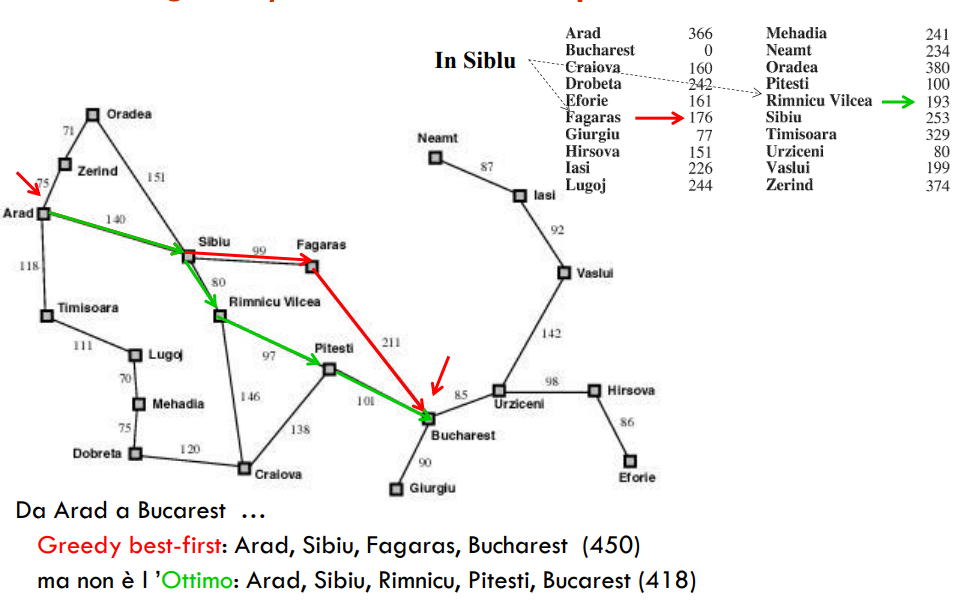
\includegraphics[scale=0.7]{greedybf.png}
\end{center}
\subsection{Algoritmo A}
Si può dire qualcosa di $f$ per avere garanzie di completezza e ottimalità?
\paragraph{Definizione} Un algoritmo A è un algoritmo Best-First con una funzione di valutazione dello stato del tipo $$f(n) = g(n) + h(n)$$ con $h(n) \geq 0$ e $h(goal) = 0$. $g(n)$ è il \textbf{costo del cammino percorso per raggiungere $n$} e $h(n)$ è \textbf{una stima del costo per raggiungere da $n$ un nodo $goal$}.
Vedremo \textbf{casi particolari} dell'algoritmo A:
\begin{list}{}{}
	\item se $h(n) = 0$, cioè $f(n) = g(n)$, si ha \textbf{Ricerca Uniforme} (UC)
	\item se $g(n) = 0$, cioè $f(n) = h(n)$, si ha \textbf{Greedy Best First}
\end{list}
\paragraph{Esempio} Il \textbf{gioco dell'otto}
\begin{multicols}{2}
\begin{center}
	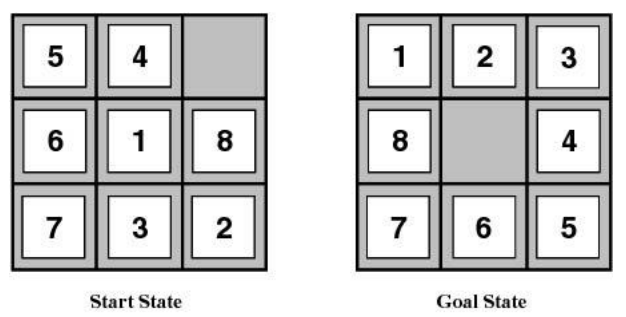
\includegraphics[scale=0.5]{8game.png}
\end{center}
\begin{list}{}{}
	\item $f(n) = $ \#mosseFatte $+$ \#caselleFuoriPosto
	\item $f(start)$ = 0 + 7\\Dopo $\leftarrow$, $\downarrow$, $\uparrow$, $\rightarrow$ si ha $f$ = 4 + 7: stesso stato ma $g$ è cambiata.
	\item $f(goal)$ = ? + 0
\end{list}
\end{multicols}
\pagebreak
\subsubsection{Algoritmo A è completo}
\paragraph{Teorema} L'algoritmo A con la condizione $g(n) \geq d(n)\cdot\epsilon$, con $d(n)$ profondità e $\epsilon > 0$ costo minimo dell'arco, è \textbf{completo}.\\
La condizione ci garantisce che non si verifichino condizioni del tipo
\begin{center}
	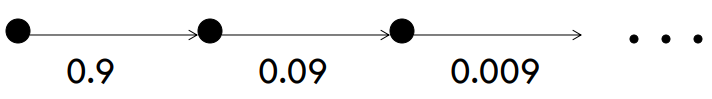
\includegraphics[scale=0.5]{complA.png}
\end{center}
e che il costo lungo un cammino non cresca "abbastanza", così da fermarsi per costi alti di $g$.
\paragraph{Dimostrazione} Sia $[n_0\:n_1\:n_2 \ldots\:n'\:\ldots\:n_k = goal]$ un cammino soluzione. Sia $n'$ un nodo della frontiera su un cammino soluzione $\rightarrow$ $n'$ prima o poi \textbf{verrà espanso}. Infatti, esistono solo un numero finito di nodi $x$ che possono essere aggiunti alla frontiera con $f(x) \leq f(n')$ (condizione su $g$).\\
Quindi, se non si trova una soluzione prima, $n'$ verrà espanso e i suoi successori aggiunti alla frontiera. Tra questi, \textbf{anche il suo successore sul cammino soluzione}.\\
Il ragionamento si può ripetere fino a dimostrare che anche il nostro $goal$ sarà selezionato per l'espansione.
\subsection{Algoritmo A*: La Stima Ideale}
Una \textbf{funzione di valutazione ideale} (\textbf{oracolo}) $f^*(n) = g^*(n) + h^*(n)$
\begin{list}{}{}
	\item $g^*(n)$ costo del \textbf{cammino minimo} da radice a $n$
	\item $h^*(n)$ costo del \textbf{cammino minimo} da $n$ a $goal$
	\item $f^*(n)$ costo del \textbf{cammino minimo} da radice a $goal$, attraverso $n$
\end{list}
Normalmente $g(n) \geq g^*(n)$ (costo del cammino $\geq$ cammino minimo) e $h(n)$ è una \textbf{stima} di $h^*(n)$: si può sotto o sovrastimare la distanza dalla soluzione.
\paragraph{Definizione} \textbf{Euristica ammissibile} $\forall n \:\:\vline\:\:h(n) \leq h^*(n)$, $h$ è una \textbf{sottostima}, ad esempio l'euristica della distanza in linea d'aria.
\paragraph{Definizione} Algoritmo A*: un algortimo A in cui $h$ è una funzione euristica ammissibile.
\paragraph{Teorema} Gli algoritmi A* sono \textbf{ottimali}.
\paragraph{Corollario} BF con passi a costo costante e UC sono \textbf{ottimali} ($h(n) = 0$)
\begin{center}
	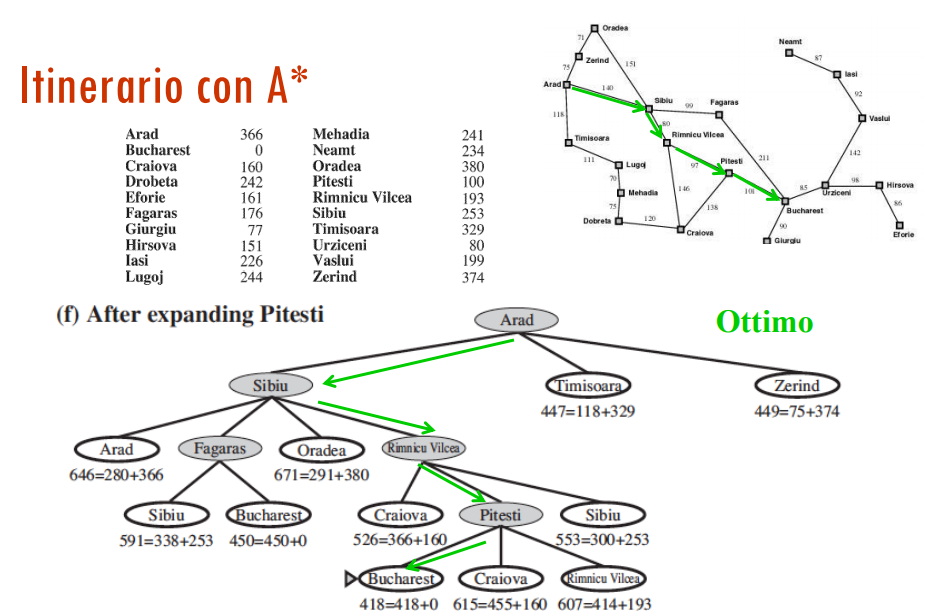
\includegraphics[scale=0.5]{itAstar.png}
\end{center}
\pagebreak
\paragraph{Osservazioni} La componente $g$ fa sì che si abbandonino cammini che vanno troppo in profondità.\\
\textbf{$h$ sotto o sovra stima}? Una sottostima può farci compiere lavoro inutile, ma \textbf{non fa perdere il cammino migliore}: quando trovo il nodo $goal$ è il cammino migliore. Invece, una funzione che a volte sovrastima può \textbf{farci perdere la soluzione ottimale a causa di tagli per sovrastima}.
\paragraph{Ottimalità} Nel caso di ricerca su ablero, l'\textbf{uso di un'euristica ammissibile è sufficiente a garantire l'ammissibilità} $\Rightarrow$ \textbf{ottimalità di A*}.\\
Nel caso di ricerca su grafo, serve una proprietà più forte: la \textbf{consistenza}, anche detta \textbf{monotonicità}, perché rischio di scartare candidati ottimi (stato già incontrato) a meno che il primo espanso sia il migliore.
\paragraph{Definizione} \textbf{Euristica consistente} se
\begin{list}{}{}
	\item $h(goal) = 0$
	\item \textbf{Consistenza locale}: $\forall n\:\:\vline\:\:h(b) \leq c(n, a, n') + h(n')$ dove $n'$ è un successore di $n$ e $c(n, a, n')$ è il costo del cammino $n\rightarrow n'$ sull'arco $a$.
	\item $\Rightarrow$ $f(b) \leq f(n')$
\end{list}
Quindi se $h$ è consistente, allora \textbf{$f$ non decresce mai lungo i cammini}: da qui il termine monotonia.\\
Esistono euristiche ammissibili che non sono monotone, ma sono rare.
\paragraph{Teorema} Un'\textbf{euristica monotona è ammissibile}.\\
Le euristiche monotone garantiscono che la \textbf{soluzione meno costosa venga trovata per prima} e quindi \textbf{sono ottimali anche nel caso di ricerca su grafo}.
\begin{list}{}{}
	\item Non si devono recuperare, tra gli antenati, nodi con costo minore
	\item \textbf{Lista degli esplorati}, stato già esplorato è sul cammino ottimo $\Rightarrow$ posso evitare di inserire il corrente ripetuto senza perdere l'ottimalità
	\begin{lstlisting}
	if (figlio.Stato non in Esplorati and non in Frontiera)
		Frontiera = Inserisci(figlio, Frontiera)
	\end{lstlisting}
	\item Per la frontiera, volendo evitare stati ripetuti, resta l'\texttt{if} finale di UC
	\begin{lstlisting}
	if (figlio.Stato in Frontiera con costoCammino piu alto)
		sostituisci quel nodo frontiera con il figlio
	\end{lstlisting}
\end{list}
\paragraph{Ottimalità di A*} \textbf{Dimostrazione}\\
\textbf{1.} $h(n)$ consistente $\Rightarrow$ i valori di $f(n)$ lungo un cammino sono non decrescenti:
\begin{list}{}{}
	\item Se $h(n) \leq c(n, a, n’) + h(n’)$ (def. consistenza)
	\item $g(n) + h(n) \leq g(n) + c(n, a, n’) + h(n’)$ sommando g(n)
	\item ma siccome $g(n) + c(n, a, n’) = g(n’)$, allora $g(n) + h(n) \leq g(n’) + h(n’)$
	\item quindi $f(n) \leq f(n’)$
\end{list}
\textbf{2.} Ogni volta che A* seleziona un nodo $n$ per l’espansione, il
cammino ottimo a tale nodo è stato trovato.\\
Se così non fosse, ci sarebbe un altro nodo $n’$ della frontiera sul cammino ottimo (a $n$, ancora da trovare), con $f(n’)$ minore (per la monotonia e n successivo di $n’$).\\
Ma ciò non è possibile perché tale nodo sarebbe già stato espanso.\\\\
\textbf{3.} Quando seleziona nodo $goal$ è cammino ottimo $[h=0, f=C^*]$
\subsection{Perché A* è vantaggioso?}
\begin{list}{}{}
	\item A* espande tutti i nodi con $f(n) < C^*$
	\item A* espande \textit{alcuni} nodi con $f(n) = C^*$
	\item \textbf{A* non espande alcun nodo con $f(b) > C^*$}
\end{list}
Quindi alcuni nodi (e suoi sottoalberi) non verranno considerati per l'espansione, ma restiamo ottimali: \textbf{pruning}, un'$h$ opportuna, \textbf{più alta possibile fra le ammissibili}, fa tagliare molto.
\pagebreak
\begin{center}
	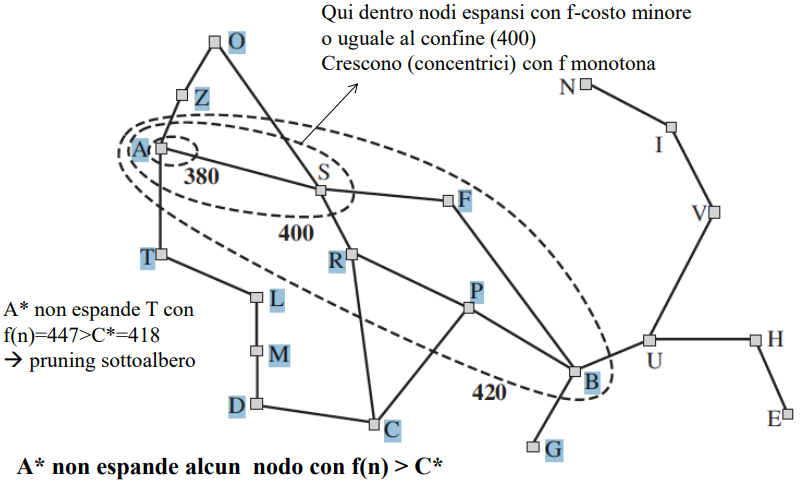
\includegraphics[scale=0.7]{astarcontorni.png}
\end{center}
Più $f$ è aderente, più taglio ottenendo ovali più stretti. Cercheremo quindi un'$h$ \textbf{più alta possibile tra le ammissibili}. Se molto bassa, molti (sino a tutti) nodi restano $< C^*$ $\Rightarrow$ espando tutti (a cerchi).
\paragraph{Pruning} Il \textbf{pruning dei sotto-alberi è il punto focale}: non li abbiamo già in memoria ed \textbf{evitiamo di generarli}, e ciò è \textbf{decisivo per i problemi di AI a spazio stati esponenziali}.
\subsection{Conslusioni su A*}
\paragraph{Algoritmo} Lo stesso usato per UC
\paragraph{Funzioni} Usa $f = g + h$ per la coda di priorità, dove $h$ e $g$ soddisfano le condizioni per algoritmo A e $h$ è una funzione euristica ammissibile per A*.\\
Sui grafi necessità di un'euristica monotona.
\paragraph{Completo} Discende dalla completezza di A, perché A* è un A particolare
\paragraph{Ottimale} Con euristica monotona
\paragraph{Ottimamente efficiente} A parità di euristica nessun'altro algoritmo espande meno nodi senza rinunciare ad ottimalità
\paragraph{Problemi} Quale euristica?\\
Occupazione in memoria: O(b$^{d+1}$)
\subsection{Casi speciali di A}
\begin{list}{}{}
	\item $h(n) = 0$ si ha Uniform Cost, cioè $f(n) = g(n)$\\
	Cioè $g$ non basta
	\item $g(n) = 0$ si ha Greedy Best First, cioè $f(n) = h(n)$\\
	Ossia $h$ non basta
\end{list}
\pagebreak
\section{Costruire le Euristiche di A*}
\subsection{Valutazione di funzioni euristiche}
A parità di ammissibilità, \textbf{una euristica può essere più efficiente di un'altra} nel trovare il cammino soluzione migliore. Questo \textbf{dipende da quanto \textit{informata} è l'euristica}, cioè dal \textbf{grado di informazione posseduto}.
\begin{list}{}{}
	\item $h(n) = 0$ \textbf{minimo} di informazione (BF, o UC)
	\item $h^*(n)$ \textbf{massimo} di informazione (oracolo)
\end{list}
In generale, per le euristiche ammissibili, $$0 \leq h(n) \leq h^*(n)$$
\paragraph{Teorema} Se $h_1 \leq h_2$, i nodi espansi da A* con $h_2$ sono un \textbf{sottoinsieme} di quelli espansi da A* con $h_1$.\\
Questo perché A* espande tutti i nodi con $f(n) < C^*$ e sono meno per $h$ maggiore (fa andare più nodi oltre $C^*$).\\
$\Rightarrow$ Se $h_1 \leq h_2$, allora A* con $h_2$ è \textbf{almeno efficiente} quanto A* con $h_1$.\\\\
Un'euristica più informata (accurata) riduce lo spazio di ricerca (più efficiente) ma è tipicamente \textbf{più costosa da calcolare}.
\subsection{Confronto di euristiche ammissibili}
\paragraph{Esempio} Due euristiche ammissibili per il gioco dell'otto
\begin{list}{}{}
	\item $h_1$ conta il numero di caselle fuori posto
	\item $h_2$ somma delle distanze Manhattan (orizz/vert) delle caselle fuori posto dalla posizione finale\\
	Manhattan Distance: $h(x, y) = MD((x, y), (x_g, y_g)) = |x - x_g| + |y - y_g|$
\end{list}
$\Rightarrow$ $h_2$ è \textbf{più informata} di $h_1$, infatti $\forall n \Rightarrow h_1(n) \leq h_2(n)$. Si dice che \textbf{$h_2$ domina $h_1$}.
\begin{center}
	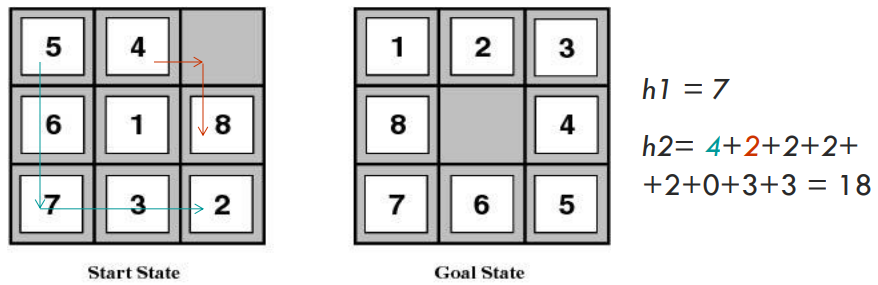
\includegraphics[scale=0.7]{confrh.png}
\end{center}
\subsection{Misura del potere euristico}
Come valutare gli algoritmi di ricerca euristica
\paragraph{Fattore di diramazione effettivo} Dato N numero di nodi generati, d profondità della soluzione, allora b* è il \textbf{fattore di diramazione di un albero uniforme con N+1 nodi}, soluzione dell'equazione $$N + 1 = b^* + (b^*)^2 + \ldots + (b^*)^d$$ Sperimentalmente, una buona euristica ha un b* abbastanza vicino ad 1 ($<$ 1.5)
\paragraph{Esempio} $d = 5,\:\: N = 52 \Rightarrow b^* = 1.92$
\pagebreak
\subsection{Capacità di esplorazione} Influenza di b*
\begin{multicols}{2}
	\begin{list}{}{Con $b = 2$}
		\item $d = 6\:\:\:\:N = 100$
		\item $d = 12\:\:N = 10000$
	\end{list}
		\begin{list}{}{Con $b = 1.5$}
		\item $d = 12\:\:N = 100$
		\item $d = 24\:\:N = 10000$
	\end{list}
\end{multicols}
Quindi \textbf{migliorando di poco l'euristica si riesce, a parità di nodi espansi, a raggiungere una profondità doppia}.
\subsection*{Quindi}
Tutti i problemi dell'IA, o quasi, sono di complessità esponenziale nel generare nodi (ad es. configurazioni possibili), ma c'è esponenziale ed esponenziale. L'euristica può migliorare di molto la capacità di esplorazione dello spazio degli stati rispetto alla ricerca cieca: \textbf{migliorando anche di poco l'euristica si riesce ad esplorare uno spazio molto più grande}.
\section{Come si inventa un'euristica?}
Alcune strategie per ottenere euristiche ammissibili, da vedere man mano:
\begin{list}{}{}
	\item \textbf{Rilassamento} del problema
	\item \textbf{Massimizzazione di euristiche}
	\item \textbf{Database di pattern disgiunti}
	\item \textbf{Combinazione lineare}
	\item \textbf{Apprendere} dall'esperienza
\end{list}
\subsection{Rilassamento del problema}
\textbf{Spazio degli stati con archi aggiunti}.
\paragraph{Gioco dell'otto} Nel gioco dell'otto, mossa da A a B possibile se \textbf{B adiacente ad A} e \textbf{B libera}.\\
$h_1$ e $h_2$ sono \textbf{calcoli della distanza esatta della soluzione} in \textbf{versioni semplificate} del puzzle: uno \textbf{spazio degli stati con archi aggiunti}
\begin{list}{}{}
	\item $h_1$ nessuna restrizione: sono sempre ammessi scambi tra caselle, si muove ovunque $\rightarrow$ numero di caselle fuori posto
	\item $h_2$ solo prima restrizione: sono ammessi spostamenti anche su caselle occupate purché adiacenti $\rightarrow$ somma delle distanze Manhattan
\end{list}
\subsection{Massimizzazione di euristiche}
Si hanno una serie di euristiche ammissibili $h_1$, $h_2$, \ldots, $h_k$, \textbf{senza che nessuna domini un'altra}. Allora conviene \textbf{prendere il massimo dei loro valori} $$h(n) = max\{h_1(n),\:\:h_2(n),\:\:\ldots,\:\:h_k(n)\}$$ Se le $h_i$ sono ammissibili, anche la $h$ lo è e \textbf{domina tutte le altre}.
\pagebreak
\paragraph{Euristiche da sottoproblemi}
\begin{center}
	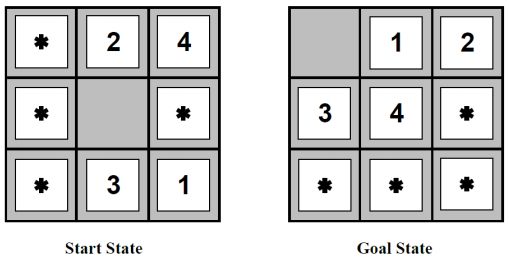
\includegraphics[scale=0.7]{eursottoprob.png}
\end{center}
Il \textbf{costo della soluzione ottima del sottoproblema} (sistemare 1, 2, 3, 4) è una \textbf{sottostima del costo del problema nel suo complesso} e più accurata della Manhattan.\\
\textbf{Database di pattern}: si \textbf{memorizza ogni istanza del sottoproblema con relativo costo} della soluzione. Si usa il \textbf{database per calcolare $h_{DB}$}, estraendo dal DB la configurazione corrispondente allo stato completo corrente.
\paragraph{Sottoproblemi multipli} Potremmo poi fare la stessa cosa per altri sottoproblemi: 5-6-7-8, 2-4-6-8\ldots ottenendo altre euristiche ammissibili.\\
Poi si può prendere il valore massimo: altra euristica ammissibile.\\
Ma potremmo sommarle ed ottenere un'euristica ancora più accurata?
\subsection{Pattern Disgiunti} In generale no, perché le \textbf{soluzioni ai sottoproblemi interferiscono}: nel caso del gioco dell'otto, condividono alcune mosse perché se sposto 1-2-3-4 sposto anche 4-5-6-7.\\
La \textbf{somma delle euristiche in generale non è ammissibile} perché potremmo sovrastimare, avendo avuto aiuti mutui.\\
Si deve \textbf{eliminare il costo delle mosse che contribuiscono all'altro sottoproblema}: \textbf{databse di \textit{pattern disgiunti}} consentono di sommare i costi (\textbf{euristiche additive}).\\
Sono molto efficaci: gioco del 15 in pochi ms. Ma difficile scomporre per il cubo di Rubik.
\subsection{Apprendere dall'esperienza}
Si fa girare il programma e si raccolgono i dati sottoforma di \textbf{coppie} \texttt{<stato, h*>}. Si usano i dati per apprendere come predire la $h$ con \textbf{algoritmi di apprendimento induttivo}: da istanze note stimiamo $h$ \textbf{in generale}.\\
Gli algoritmi di apprendimento si concentrano su caratteristiche salienti dello stato (\textit{feature}, $x_i$). Esempio: numero tasselli fuori posto 5 $\rightarrow$ costo 14.
\subsubsection{Combinazione di euristiche}
Quando diverse caratteristiche influenzano la bontà di uno stato, si può usare una combinazione lineare $$h(n)= c_1 x_1(n) + c_2 x_2(n) + \ldots + c_k x_k(n)$$
Gioco dell'otto $h(n) = c_1 \#fuoriPosto + c_2 \#coppieScambiate$\\
Scacchi $h(n) = c_1 vantaggioPezzi + c_2 pezziAttaccante + c_3 regina + \ldots$\\
Il \textbf{peso dei coefficienti può essere aggiustato con l'esperienza}, anche qui \textbf{apprendendo automaticamente da esempi di gioco}. $h(goal) = 0$ ma ammissibilità e consistenza \textbf{non} automatiche.

\chapter{Algoritmi Evolutivi Basati su A*}
\section{Beam Search}
Nel \textbf{best first} viene mantenuta tutta la frontiera. Se l'occupazione di memoria è eccessiva, si può ricorrere ad una variante: la \textbf{beam search}.
\paragraph{Beam Search} La beam search \textbf{tiene ad ogni passo solo i $k$ nodi più promettenti}, dove $k$ è detto \textbf{ampiezza del raggio} (beam).\\
\textbf{Non è completa}.
\section{IDA*}
A* con approfondimento iterativo. IDA* combina A* con ID: ad ogni iterazione si ricerca in profondità con un limite (cut-off) dato dal valore della funzione $f$ (e non dalla profondità).\\
Il limite \textbf{f-limit} viene aumentato ad ogni iterazione, fino a trovare la soluzione.
\paragraph{Punto Critico} Di quanto viene aumentato f-limit.
\paragraph{Quale incremento?} Cruciale la scelta dell'incremento per garantire l'ottimalità. In caso di azioni dal costo fisso, il limite viene incrementato dal costo delle azioni.\\
Ma in caso di costi variabili? Costo minimo? Si potrebbe, ad ogni passo, fissare il limite successivo al valore minimo delle $f$ scartate (in quanto superavano il limite) all'interazione precedente.
\paragraph{Analisi} \textbf{Completo} e \textbf{ottimale}. Occupazione in memoria O(bd).
\section{RBFS}
Best-First Ricorsivo: simile a DF ricorsivo ma cerca di usare meno memoria, facendo del lavoro in più.\\
Tiene traccia del migliore percorso alternativo ad ogni livello. Invece di fare backtracking in caso di fallimento, interrompe l’esplorazione quando trova un nodo meno promettente secondo $f$. Nel tornare indietro \textbf{si ricorda il miglior nodo che ha
trovato nel sottoalbero esplorato}, per poterci eventualmente tornare\\
Memoria: lineare nella profondità della soluzione ottima.
\section{A* con memoria limitata}
L'idea è quella di utilizzare al meglio la memoria disponibile.\\
SMA* procede come A* fino ad esaurimento della memoria disponibile. A questo punto “dimentica” il nodo peggiore, dopo avere aggiornato il valore del padre.\\
A parità di $f$ \textbf{si sceglie il nodo migliore più recente e si dimentica il nodo peggiore più vecchio}.\\
\textbf{Ottimale se il cammino soluzione sta in memoria}.\\
\pagebreak

In algoritmi a memoria limitata, le limitazioni della memoria possono portare a compiere molto lavoro inutile: ad esempio, visitare ripetutamente gli stessi nodi. Diventa quindi \textbf{difficile stimare la complessità temporale effettiva}. Le \textbf{limitazioni della memoria}, quind, \textbf{possono rendere un problema intrattabile} dal punto di vista computazionale.
\section{Conclusioni}
\begin{list}{}{}
	\item \textbf{Agenti} in \textbf{ambienti deterministici}, \textbf{osservabili}, \textbf{statici} e \textbf{completamente noti}
	\item \textbf{Ricerca} come \textbf{scelta della sequenza di azioni}, cioè cammino in uno spazio di stati, \textbf{che raggiunge obiettivo} $\Rightarrow$ il cammino è la soluzione
	\item \textbf{Attività necessarie}
	\begin{list}{}{}
		\item Formulazione del problema
		\item Scelta dell'algoritmo di ricerca adeguato
		\item Identificazione della funzione di valutazione euristica più efficace
	\end{list}
\end{list}
\chapter{Oltre la Ricerca Classica}
\paragraph{Risolutori "classici"} Gli agenti risolutori di problemi \textit{classici} assumono le condizioni viste in precedenza:
\begin{list}{}{}
	\item Ambienti completamente osservabili
	\item Ambienti deterministici
	\item Si trovano nelle condizioni di produrre un piano d'azione eseguibile "ad occhi chiusi": possono studiare la sequenza d'azioni \textit{offline}, che può essere eseguita senza imprevisti per raggiungere l'obiettivo
\end{list}
\section{Verso ambienti più realistici} La \textbf{ricerca sistematica}, o euristica, nello spazio di stati è \textbf{troppo costosa} $\longrightarrow$ Metodi di ricerca locale\\
Assunzioni sull'ambiente da considerare:
\begin{list}{}{}
	\item \textbf{Azioni non deterministiche}\\
	\textbf{Ambiente parzialmente osservabile}\\
	$\longrightarrow$ Piani condizionali, ricerca \texttt{AND-OR}, stati credenza
	\item \textbf{Ambienti sconosciuti}\\
	\textbf{Problemi di esplorazione} (percezioni forniscono nuove informazioni dopo l'azione)\\
	$\longrightarrow$ Ricerca \textbf{online}
\end{list}
\section{Ricerca Locale}
\paragraph{Assunzioni}
Gli algoritmi visti fin'ora esplorano gli spazi degli stati alla ricerca di un goal e restituiscono un \textbf{cammino soluzione}, ma \textbf{a volte lo stato goal è la soluzione} del problema. Gli \textbf{algoritmi di ricerca locale} sono adatti per problemi in cui
\begin{list}{}{}
	\item La sequenza di azioni non è importante: quello che conta è lo stato goal
	\item Tutti gli elementi della soluzione sono nello stato ma alcuni vincoli sono violati
\end{list}
\subsection{Algoritmi di ricerca locale}
\begin{list}{}{}
	\item \textbf{Non sono sistematici}
	\item Tengono traccia solo del nodo corrente e si spostano su nodi adiacenti
	\item Non tengono traccia dei cammini, poiché non servono a lavoro finito
	\begin{list}{}{}
		\item Efficienti in memoria
		\item Possono trovare soluzioni ragionevoli anche in spazi molto grandi o infiniti, come nel caso di spazi continui
	\end{list}
	\item Utili per \textbf{risolvere problemi di ottimizzazione}
	\begin{list}{}{}
		\item \textbf{Stato migliore secondo una funzione obiettivo}
		\item Stato di costo minore
		\item Esempio: training di un modello di Machine Learning
	\end{list}
\end{list}
\pagebreak
\subsection{Panorama dello spazio degli stati}
Esempio di una $f$ euristica di costo della funzione obiettivo (non del cammino)
\begin{center}
	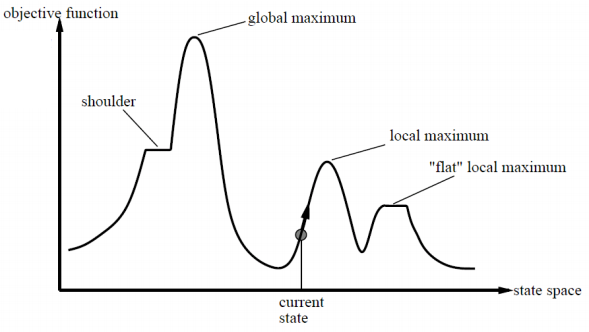
\includegraphics[scale=1]{statesspace.png}
\end{center}
Uno \textbf{stato ha una posizione sulla superficie} e un'\textbf{altezza corrispondente al valore della sua funzione di valutazione}. Un \textbf{algoritmo provoca un movimento sulla superficie}.\\
Trovare \textbf{avvallamento più basso} (es: costo minimo) \textbf{o il picco più alto} (es: massimo di un obiettivo)
\subsection{Algoritmo Hill Climbing}
Anche detto \textbf{ricerca in salita}, \textbf{steepest ascent/descent}.\\
Ricerca locale \textbf{greedy}.\\
Vengono generati i successori e valutati. Viene scelto un nodo che migliora la valutazione dello stato attuale (\textbf{non si tiene traccia degli altri}, quindi non ho l'albero di ricerca in memoria). La scelta del nodo dipende dall'algoritmo:
\begin{list}{}{}
	\item Migliore $\rightarrow$ \textbf{Hill Climbing a salita ripida}
	\item Uno a caso tra quelli che migliorano $\rightarrow$ \textbf{Hill Climbing Stocastico}
	\item Il primo $\rightarrow$ \textbf{Hill Climbing con prima scelta}
\end{list}
Se non ci sono stati migliori, l'algoritmo termina con \textbf{fallimento}.
\begin{lstlisting}
function Hill-climbing(problema) returns stato-massimo-locale
  nodo-corrente = CreaNodo(problema.Stato-iniziale)
  loop do
    vicino = successore di nodo-corrente di valore piu alto
    if (vicino.Valore <= nodo-corrente.Valore)
      return nodo-corrente.Stato #interrompe la ricerca
    nodo-corrente = vicino #altrimenti, se vicino migliore, continua
\end{lstlisting}
Si prosegue solo se il vicino più alto è migliore dello stato corrente, se tutti i vicini sono peggiori, si ferma. Non c'è frontiera a cui tornare, si tiene solo uno stato.\\
Tempo: numero di cicli variabile in base al punto di partenza.
\pagebreak
\paragraph{Problema delle 8 Regine} Con formulazione a stato completo
\begin{multicols}{2}
\begin{list}{}{}
	\item Costo $h$ $=$ numero di coppie di regine che si attaccano a vicenda
	\item I numeri sono i valori dei successori (7 $\times$ 8, 7 posizioni per ogni regina = su ogni colonna)
	\item Tra i migliori (valore 12) si \textbf{sceglie a caso}
	\item Minimo globale = 0
\end{list}
\begin{center}
	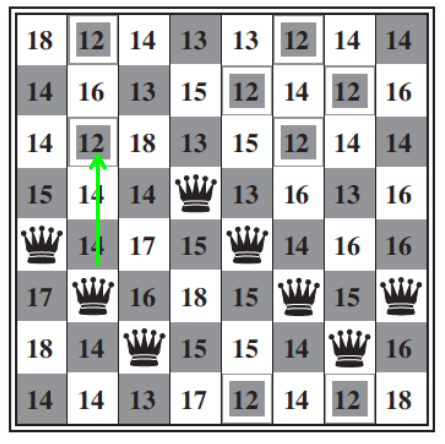
\includegraphics[scale=0.6]{8regstatcomp.png}
\end{center}
\end{multicols}
\begin{multicols}{2}
\begin{center}
	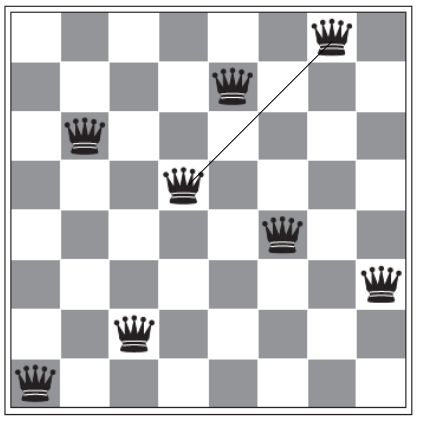
\includegraphics[scale=0.6]{8regstatcomp2.png}
\end{center}
\begin{list}{}{\textbf{Un minimo locale}}
		\item $h$ = 1
		\item Tutti gli stati successori non migliorano la situazione (minimo locale)
		\item \textbf{Per le 8 regine Hill-Climbing si blocca l'86\% delle volte}\\
		Ma in media sono 4 passi per la soluzione, e 3 quando si blocca
		\item Su $8^8$ = 17 milioni di stati
\end{list}
\end{multicols}
\paragraph{Esempio} Successo in tre mosse\\
$h$ qui è l'\textbf{euristica di costo della funzione obiettivo} da minimizzare
\begin{center}
	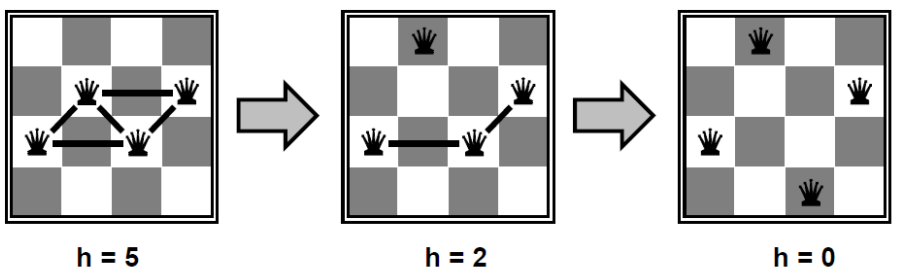
\includegraphics[scale=0.75]{8regine3passi.png}
\end{center}
\pagebreak
\subsubsection{Problemi con Hill-Climbing}
Se la funzione è da ottimizzare, i picchi sono massimi locali o soluzioni ottimali. Nel grafico si possono presentare: \textbf{massimi locali}, \textbf{plateu} (pianori), \textbf{spalle} e \textbf{crinali}/creste.
\paragraph{Miglioramenti}
\begin{enumerate}
	\item Consentire un \textbf{numero limitato di mosse laterali}\\
	Ossia ci si ferma per $<$ nell'algoritmo, anziché per $\leq$\\
	$\Rightarrow$ L'algoritmo sulle 8 regine ha successo nel 94\% dei casi, ma impiega in media 21 passi
	\item Hill-Climbing Stocastico: si \textbf{sceglie a caso tra le mosse in salita}, magari tenendo conto della pendenza.\\
	Converge più lentamente ma a volte trova soluzioni migliori
	\item Hill-Climbing con prima scelta: può generare le mosse a caso fino a trovarne una migliore dello stato corrente. Più \textbf{efficace quando i successori sono molti} (es: migliaia)
	\item Hill-Climbing con riavvio casuale (\textbf{random restart}): ripartire da un punto scelto a caso.\\
	Se la probabilità di successo è $p$, saranno necessarie in media $\frac{1}{p}$ ripartenze per trovare la soluzione (Es.: 8 regine, $p$ = 0.14, 7 iterazioni cioè 6 fallimenti e un successo).\\
	\textbf{Tendenzialmente completo}: insistendo si generano tutte le possibilità.\\
	Per le regine, 3 milioni di regine in meno di un minuto. Se funziona o no dipende molto dalla forma del panorama degli stati.
\end{enumerate}
\subsection{Algoritmo di Tempra Simulata}
\paragraph{Simulated Annealing} L'algoritmo di tempra simulata combina Hill-Climbing con una scelta stocastica ma \textbf{non del tutto casuale perché poco efficiente}. L'analogia è col processo di tempra dei metalli: portati a temperature molto elevate e raffreddati gradualmente consentendo di cristallizzare in uno stato a più bassa energia.
\paragraph{Tempra Simulata} Ad ogni passo si \textbf{sceglie un successore a caso}:
\begin{list}{}{}
	\item Se migliora lo stato corrente, viene espanso
	\item Se non lo migliora (caso in cui $\Delta E = f(n') - f(n) < 0$), quel nodo viene scelto con probabilità $p = e^{\Delta E/T}$, con $p$ ovviamente $0 \leq p \leq 1$\\
	(Si genera un numero casuale tra 0 e 1, se questo è $<$ $p$ il successore viene scelto, altrimenti no)
	\item $p$ è \textbf{inversamente proporzionale al peggioramento}
	\item $T$ (\textbf{temperatura}) \textbf{decresce al progredire dell'algoritmo}, quindi anche $p$, \textbf{secondo un piano definito}.\\
	Col progredire, rende improbabili le mosse peggiorative.
\end{list}
\paragraph{Analisi} La probabilità di una mossa in discesa diminuisce col tempo, e l'algoritmo si comporta sempre di più come Hill-Climbing.\\
Se $T$ viene decrementato abbastanza lentamente, con probabilità tendente ad 1 si raggiunge la soluzione ottimale.\\
\textbf{Analogia}: $T$ corrisponde alla temperatura e $\Delta E$ alla variazione di energia
\paragraph{Parametri} \textbf{Valore iniziale} e \textbf{decremento di $T$} sono parametri.\\
I valori per $T$ sono \textbf{determinati sperimentalmente}: il \textbf{valore iniziale di $T$} è \textbf{tale che per valori medi di $\Delta E$}, $p = e^{\Delta E/T}$ sia circa 0.5
\subsection{Algoritmo Local Beam}
Versione locale della beam search.\\
Si tengono in memoria $k$ stati invece che uno solo. Ad ogni passo si generano i successori di tutti i $k$ stati.
\begin{list}{}{}
	\item Se si trova un goal, ci si ferma
	\item Altrimenti si prosegue con i $k$ migliori tra questi
\end{list}
Note:
\begin{list}{}{}
	\item Diverso da K restart (che riparte da 0)
	\item Diverso da beam search
\end{list}
\pagebreak
\subsection{Algoritmo Beam Search Stocastico}
Si introduce un elemento di casualità, come in un processo di selezione naturale: \textbf{diversificare la nuova generazione}.\\
In questa variante stocastica, si scelgono $k$ successori ma \textbf{con probabilità maggiore per i migliori}. \textbf{Terminologia}:
\begin{list}{}{}
	\item \textbf{Organismo}, stato
	\item \textbf{Progenie}, successori
	\item \textbf{Fitness} (valore della $f$), idoneità
\end{list}
\section{Algoritmi Genetici}
\paragraph{L'Idea} Sono \textbf{varianti della beam search stocastica} in cui gli \textbf{stati successori sono ottenuti \textit{combinando} due stati genitore} anziché per evoluzione. \textbf{Terminologia}:
\begin{list}{}{}
	\item \textbf{Popolazione} di \textbf{individui} (stati)
	\item \textbf{Fitness}
	\item \textbf{Accoppiamenti} e \textbf{mutazione genetica}
	\item \textbf{Generazioni}
\end{list}
\paragraph{Funzionamento} \textbf{Popolazione iniziale}: $k$ stati/\textbf{individui} generati casualmente. Ogni \textbf{individuo è rappresentato come una stringa}: ad esempio 24 bit, o posizione nelle colonne ("\textit{24748552}") per le 8 regine.\\
Gli \textbf{individui} sono \textbf{valutati da una funzione di fitness}: ad esempio numero di coppie di regine che \textit{non} si toccano.\\
Si \textbf{selezionano gli individui per gli accoppiamenti}, con una probabilità proporzionale alla fitness. Le \textbf{coppie danno vita alla generazione successiva}: combinando materiale genetico (\textbf{crossover}) o con un meccanismo aggiuntivo di \textbf{mutazione genetica} (\textbf{casuale}).\\
La popolazione ottenuta dovrebbe essere migliore e la cosa si \textbf{ripete fino ad ottenere stati abbastanza buoni} (\textbf{stati obiettivo}).
\paragraph{Esempio}
\begin{center}
	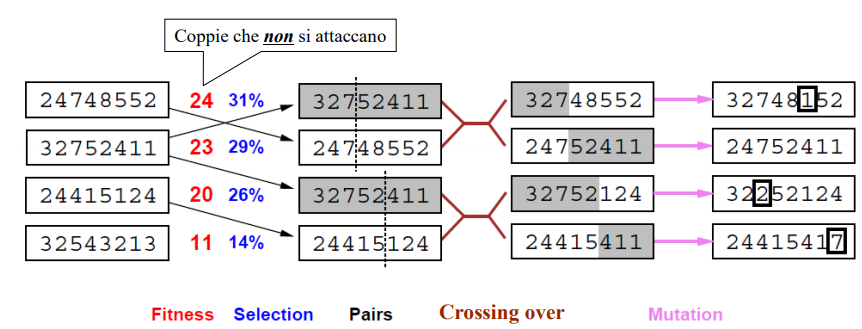
\includegraphics[scale=0.7]{alggenetic.png}
\end{center}
Per ogni coppia viene scelto un punto di \textbf{crossing over} (la linea tratteggiata) e vengono \textbf{generati due figli scambiandosi dei pezzi} \textit{del DNA}.\\
Viene infine effettuata una mutazione casuale che dà luogo alla prossima generazione.
\pagebreak
\paragraph{Nascita di un figlio}
\begin{center}
	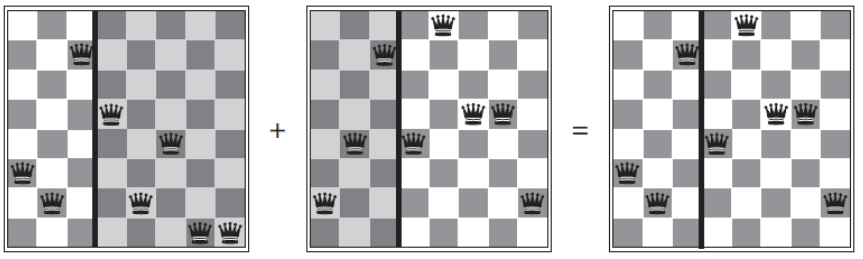
\includegraphics[scale=0.7]{8reggeneticfigli.png}
\end{center}
Le parti chiare sono passate al figlio, le parti scure si perdono. Se i genitori sono molto diversi, anche i nuovi stati sono diversi. All'inizio spostamenti maggiori che poi si raffinano.
\subsection*{Algoritmi Genetici}
\paragraph{Suggestivi} Area del \textbf{Natural Computing}. Usati molto in problemi reali (es.: configurazione di circuiti e scheduling dei lavori).\\
Combinano la tendenza a salire della beam search stocastica con l'interscambio di informazioni tra thread paralleli di ricerca (blocchi utili che si combinano).\\
Funziona meglio de il problema (soluzioni) ha componenti significative rappresentate in sottostringhe.\\
\textbf{Punto critico}: rappresentazione del problema in stringhe.
\paragraph{Spazi Continui} Molti casi reali hanno spazi di ricerca continua, fondamentale per il Machine Learning! Lo stato è descritto da variabili continue $x_1$, \ldots, $x_n$ (vettore $x$), ad esempio la posizione in uno spazio 3D $x = (x_1, x_2, x_3)$.\\
Apparentemente è complicato: fattori di ramificazione infiniti con gli approcci precedenti. Ma in realtà ci sono molti strumenti matematici per spazi continui, che portano ad approcci anche molto efficienti.
\subsection{Gradient}
Se la $f$ è \textbf{continua} e \textbf{differenziabile}, ad esempio quadratica rispetto il vettore $x$, allora il minimo/massimo lo si può cercare utilizzando il \textbf{gradiente}, che \textbf{restituisce la direzione di massima pendenza del punto}.\\
Data $f$ obiettivo $$\nabla f = \left( \frac{\partial f}{\partial x_1}, \frac{\partial f}{\partial x_2}, \frac{\partial f}{\partial x_3} \right)$$
\textbf{Hill-Climbing iterativo}: $x_{new} = x_{old} + \eta\nabla f(x)$ con $\eta$ dimensione dello step.\\
Quantifica lo spostamento, senza cercarlo tra gli infiniti possibili successori.\\
\textbf{Nota}: in generale non è sempre necessario il min/max assoluto. Vedremo nel ML.
\begin{center}
	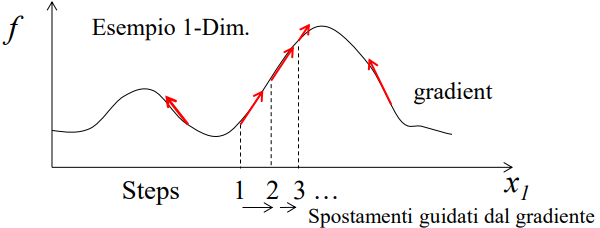
\includegraphics[scale=1]{gradient.png}
\end{center}
\pagebreak
\section{Ambienti più realistici}
\paragraph{Problemi classici} Gli agenti risolutori di problemi "classici" assumono:
\begin{list}{}{}
	\item Ambienti \textbf{completamente osservabili}
	\item Azioni e ambienti \textbf{deterministici}
	\item Piano generato è sequenza di azioni \textbf{eseguibile ad occhi chiusi}, generato \textit{offline} ed eseguito senza imprevisti
	\item Le \textbf{percezioni non servono}, se non nello stato iniziale
\end{list}
\paragraph{Soluzioni più complesse} In un ambiente \textbf{parzialmente osservabile} e \textbf{non deterministico} le \textbf{percezioni sono importanti}: \textbf{restringono gli stati} possibili e \textbf{informano} sull'effetto dell'\textbf{azione}.\\
Più che un piano, l'\textbf{agente elabora una strategia} che \textbf{tiene conto delle diverse eventualità}: un \textbf{piano con contingenza}. Esempio: aspirapolvere con assunzioni diverse.
\subsection{Azioni non deterministiche}
\paragraph{Aspirapolvere imprevedibile} Ci sono più stati possibili come risultato dell'azione.\\
\textbf{Comportamento}: se aspira in una stanza sporca la pulisce\ldots ma \textbf{a volte} pulisce anche una stanza adiacente. Se aspira in una stanza pulita, \textbf{a volte} rilascia sporco.
\paragraph{Variazioni necessarie al modello} Il modello di transizione, quindi, \textbf{restituisce un insieme di stati}: l'agente non sa in quale si troverà. Il \textbf{piano di contingenza} sarà un piano condizionale e magari con cicli.
\paragraph{Esempio}
\begin{multicols}{2}
Nell'esempio\\\texttt{Risultati(Aspira, 1) = \{5, 7\}}, cioè aspirando nello stato \texttt{1} posso finire nello stato \texttt{5} o \texttt{7}.\\
Un possibile piano è
\begin{lstlisting}
[Aspira,
	if (stato = 5):
		[Destra, Aspira]
	else:
		[]
]
\end{lstlisting}
Da sequenza di azioni a piano (albero)
\begin{center}
	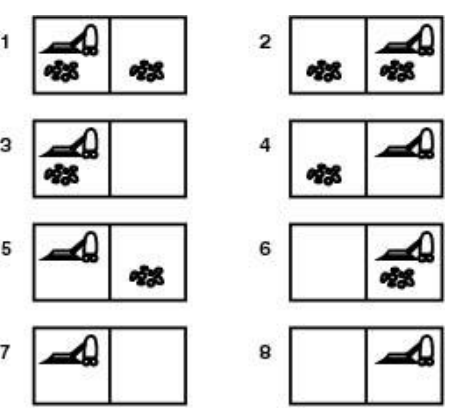
\includegraphics[scale=0.7]{aspirapolvereimprevedibile.png}
\end{center}
\end{multicols}
\subsection{Come si pianifica}
\paragraph{Alberi di Ricerca \texttt{AND-OR}}
\begin{list}{}{}
	\item Nodi \texttt{OR}: scelte dell'agente (1 sola azione)
	\item Nodi \texttt{AND}: le diverse contingenze (scelte dell'ambiente, più stati possibili), \textbf{da considerare tutte}
\end{list}
Una \textbf{soluzione ad un problema di ricerca \texttt{AND-OR}} è un \textbf{albero} che
\begin{list}{}{}
	\item Ha un nodo obiettivo in ogni foglia
	\item Specifica un'unica azione nei nodi \texttt{OR}
	\item Include tutti gli archi uscenti da nodi \texttt{AND}
\end{list}
\pagebreak
\paragraph{Esempio}
\begin{center}
	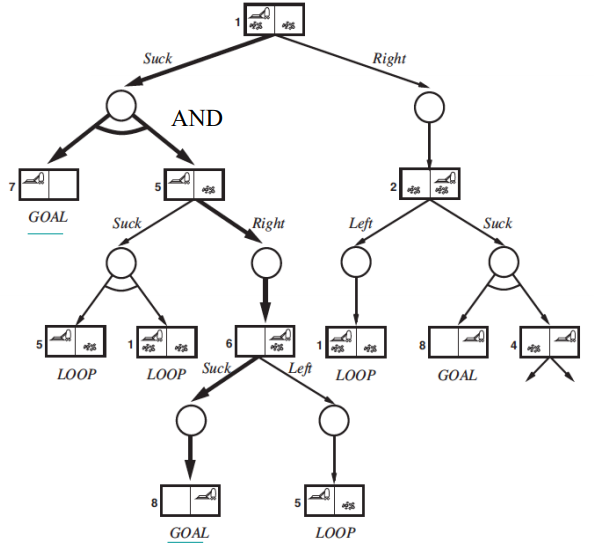
\includegraphics[scale=0.7]{andortree.png}
\end{center}
\textbf{Archi in grassetto} = soluzione (sottoalbero), la seguente:
\begin{lstlisting}
	Piano: [Aspira: if (stato = 5): [Destra, Aspira] else: []]
\end{lstlisting}
%https://elearning.di.unipi.it/pluginfile.php/30593/mod_resource/content/0/5-2020-oltre_ricerca_classica.pdf, p.38
\chapter{I Giochi con Avversario}
\paragraph{Premessa}
Fin'ora abbiamo avuto \textit{Problemi Solving} come ricerca. Il paradigma di base era: ambiente osservabile, deterministico, utente singolo e stati atomici.\\
Da adesso rilassamento delle assunzioni di base: ambiente multi agente e rappresentazioni degli stati più complesse.\\
Ci occuperemo di \textbf{specializzazioni} del paradigma: giochi con avversario. I piani quindi devono tenere conto dell'avversario.\\
Vedremo \textbf{problemi di soddisfacimento di vincoli}, sempre come ricerca in spazio di soluzioni, con stato a struttura \textbf{fattorizzata}.\\
Questo ci porterà a considerare sistemi basati su conoscenza: lo stato è una "base di conoscenza" a cui rivolgere domande rappresentato in linguaggio espressivo. Tecniche di "ragionamento" con inferenze: logica del prim'ordine e calcolo proposizionale.
\section{Giochi con Avversario}
\begin{list}{}{}
	\item Regole semplici e formalizzabili
	\item Ambiente accessibile e deterministico
	\item Due giocatori, a turni alterni, a \textbf{somma zero} (se uno vince, l'altro perde: sommare i punteggi dà 0 o risultato costante), a informazione perfetta (tutti i gioc conoscono stato gioco)
	\item Ambiente multi-agente competitivo: presenza avversario rende ambiente strategio, più difficile rispetto a visto fin'ora
	\item Complessità e vincoli di tempo reale: mossa migliore nel tempo disponbile
\end{list}
$\Rightarrow$ giochi più simili a prob reali
\section{Ciclo \textit{pianifica-agisci-percepisci}}
\paragraph{Due agenti a turno} Si può pianificare considerando le possibili risposte dell'avversario e le possibili risposte a quelle risposte\ldots\\
Una volta decisa la mossa
\begin{list}{}{}
	\item Si esegue la mossa
	\item ...
\end{list}
\section{Giochi come problemi di ricerca}
\begin{list}{}{}
	\item Stati: config gioco\\
	Player(s) a chi tocca muovere nello stato s
	\item Stato iniziale: config iniziale gioco
	\item Actions(s) mosse legali in s
	\item Result(s, a) stato risultatne da una mossa
	\item Terminal-Test(s) determina se stato è fine del gioco
	\item Utility(s, p) utilità (o pay-off) valore numerico degli stati terminali del gioco per p\\
	Es: 1, -1, 0, conteggio punti\ldots
\end{list}
\section{Algoritmo Min-Max}
Valuto stati terminali in base a punteggio/vittoria e valuto stati preterminali valutandoli in base a se mi portano a vittoria o meno a ritroso. Valuto stati intermedi con valore minimo tra gli stati risultanti.
\begin{center}
	Immagine tic-tac-toe
\end{center}
\paragraph{Valore minmax}
minimax(s) = 
\begin{list}{}{}
	\item se Terminal-Test(s) , allora Utility(s, MAX)
	\item se Player(s) = MAX , allora max$_{a \in Action(s)}$ Minimax(Result(s, a))
	\item se Player(s) = MIN , allora min$_{a \in Action(s)}$ Minimax(Result(s, a))
\end{list}
\paragraph{Come conviene esplorare l'albero di gioco?} In profondità, perché hanno ampiezza esponenziale.
\paragraph{Algoritmo ricorsivo}\ldots
\section{Algoritmo Min-Max Euristico (con orizzonte)}
Casi complessi in cui esplorare stati è troppo costoso (es. scacchi): occorre \textbf{funzione di valutazione euristica}.\\
Strategia: guardare avanti $d$ livelli\ldots

\section{Funzione di Valutazione}
Stima dell'utilità attesa a partire da una certa posizione. La qualità della funzione è determinante.
\begin{list}{}{}
	\item deve esser consistente con l'utilità se applicata a steati terminali del gioco (indurre lo stesso ordinamento)
	\item dev'essere efficiente da calcolare
	\item deve riflettere le probabilità effettive di vtitoria (A valutato meglio di B se da A ho più probabilità di vittoria rispetto a B)
	\item \ldots
\end{list}
Esempio scacchi
\paragraph{Problemi Noti}
\begin{list}{}{}
	\item \textbf{Stati Non Quiescienti}: esplorazione fino ad un livello può mostrare situaz. molto vantaggiosa, ma a mossa successiva es. regina mangiata dalla torre. Si possono riconoscere-\\
	\textbf{Soluzione}: non fermarsi a stati quiescienti ma esplorare un po' di più fino ad arrivare a stati in cui funz. valutazione non attende variazioni repentine (stati quiescienti)
	\item \textbf{Effetto Orizzonte}: si privilegiano mosse diversive che hanno solo l'effetto di spingere il problema oltre, per evitare mosse disastrose che alla fine devono accadere
\end{list}
\subsection{Ottimizzazione}
Dobbiamo esplorare ogni cammino? No esistono tecniche di potatura che dimezzano la ricerca pur mantenendo decisione min-max corretta (potatura alfa-beta)
\paragraph{Potatura Alfa-Beta} ridurre spazi ricerca algoritmi min-max
\subsection{Algoritmo Alfa-Beta}
\paragraph{Algoritmo}\ldots
\paragraph{Ordinamento delle mosse}
\paragraph{Giochi Multiplayer} Invece di aver due valori ho un vettore di valori per nodo. Per propagare all'indietro prendo vettore che migliora la valutazione.
\section{Problemi di Soddisfacimento di Vincoli}
\paragraph{CSP}
caso particolare dei problemi di ricerca, grazie alla struttura si cerca meglio la soluzione.\\
Classe ampia, esistono euristiche generali da applicare che consentono risoluzioni di dimensioni significative.\\
\paragraph{Tre componenti} \ldots
%TODO
\par\noindent\rule{\textwidth}{0.4pt}
\paragraph{Backtracking ricorsivo per CSP}
Soluzione: trovare assegnamento per le variabili con valori dal dominio per arrivare ad assegnamento completo (tt var con valori) e consistente (soddisfa vincoli)\\
Scelta dei valori: scegliere il valore meno vincolante, quello che esclude meno valori possibili per le altre variabili. Meglio valutare prima assegnamento che ha più probabilità di successo.
\paragraph{Propagazione dei vincoli}
\begin{list}{}{}
	\item \textbf{Verifica in avanti}, Forward Checking: meno costosa, una volta assegn valore vado a vedere variabili direttamente collegate nel grafo dei vincoli
	\item \textbf{Consistenza di nodo e d'arco}: più costosa ma anche più efficace, restringono valori domini variabili tenendo conto vincoli unari e binari su tutto il grafo (itero finché tutti nodi e archi sono consistenti)
\end{list}
\paragraph{Esempio di FC} (Forward Check) Colorare mappa con Rosso, Verde, Blu.
\begin{center}
	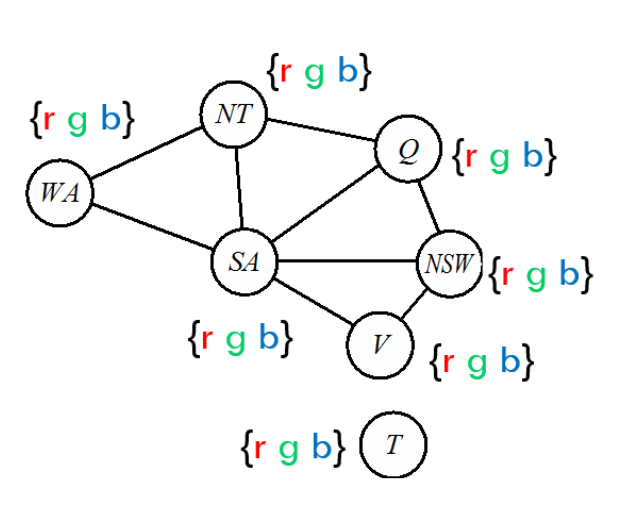
\includegraphics[scale=0.7]{FC_es1.png}
\end{center}
%TODO
\pagebreak
\paragraph{Backtracking Cronologico}
Suppongo di avere \{Q=R, NSW=G, V=B, T=R\}. Cerco di assegnare SA, il fallimento genera un backtracking cronologico: si provano tutti i valori alternativi per l'ultima variabile, T, continuando a fallire\ldots\\
Questo perché non è la T responsabile del fallimento ma le altre variabili.\\
Quindi si può fare un backtracking "intelligente" guidato dalle dipendenze.
\paragraph{Backtracking guidato dalle dipendenze} Considero le alternative solo per le variabili che hanno causato il fallimento \{Q, NSW, V\}, l'\textbf{insieme dei conflitti}.
\paragraph{Metodi CSP locali} I problemi CSP possono essere affrontati con metodi locali. Esempio: \textbf{le regine}.\\
\textbf{Euristica dei conflitti minimi} (\textbf{min-conflicts}): si sceglie un valore che crea meno conflitti. Solitamente si sceglie a caso una delle regie che violano dei vincoli.\\
Molto efficace: 1 milione di regine in 50 passi!
\begin{center}
	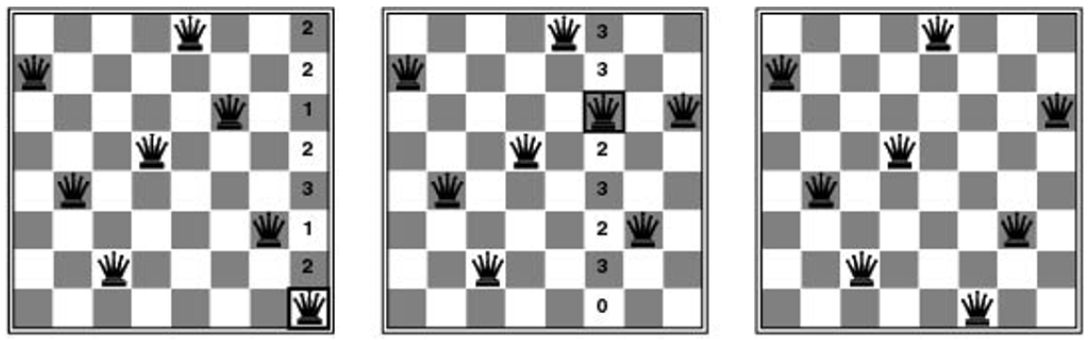
\includegraphics[scale=0.5]{minconflicts_es.png}
\end{center}
\paragraph{Conclusioni} Abbiamo visti due domini specifici per paradigma risoluzione problemi ricerca: giochi con avversario (complicazione: ambiente strategico e vincoli di tempo reale, non posso pianificiare azioni da eseguire "a occhi chiusi") e CSP (grazie a rappresenztazione stato più ricca tecniche problem solving specializzabili e usate per risolvere istanze di problemi di dimensioni maggori)\\
Prossimamente: \textbf{sistemi basati su conoscenza}. Conoscenza implica capacità inferenziali, con rappresentazione stato ancora più ricco con linguaggio rappresentazione conoscenza. L'inferenza è anch'essa un problema di ricerca in uno spazio di stati.
\chapter{Agenti Basati su Conoscenza}
Come costruire agenti dotati di capacità inferenziali.\\
Cerchiamo di migliorare capcità di ragionamento, dotando di rappresentazione del mondo più complessi non descrivibili semplicemente. Agenti basati su conoscenza, con all'interno una base di conoscenza KB con conoscenza espressa in forma esplicita e dichiarativa attraverso un linguaggio.
\begin{center}
	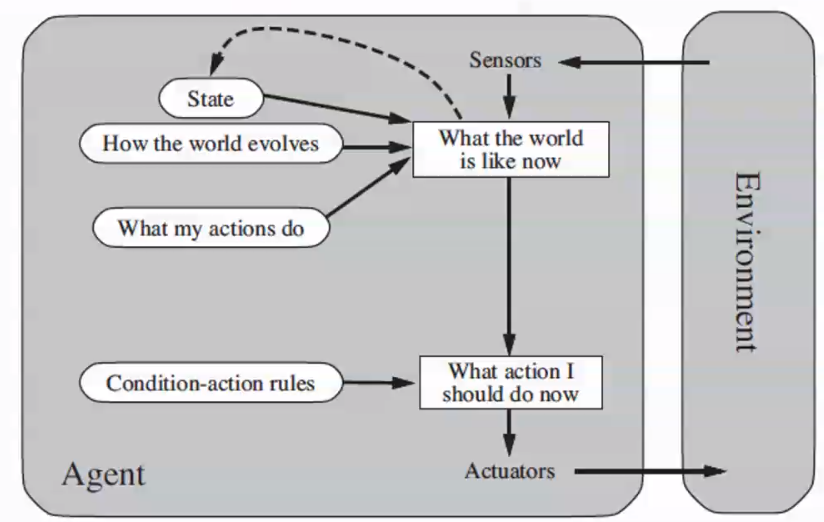
\includegraphics[scale=0.7]{ag_conosc.png}
\end{center}
La maggiorparte prob I.A. sono "\textit{knowledge-intensive}". Mondo tipicamente complesso: serve rappresentazione parziale e incompleta (astrazione) del mondo utile agli scopi dell'agente.\\
Per ambienti parzialmente osservabili e complessi ci servono linguaggi di rappresentazione della conoscenza più espressivi e capacità inferenziali.\\
La conoscenza può essere codificata a mano, acquisita o estratta da testi ed esperienza.
\paragraph{Approccio dichiarativo vs procedurale}
tipicamente conoscenza in KB in forma dichiarativa. Alternativa è codificare conoscenza in maniera procedurale con programma che implementa processo decisionale. Un agente KB (con conoscenza dichiarativa) è più flessibile: perché più semplice ricevere conoscenza in maniera incrementale e modificare il comportamento con l'esperienza.
\pagebreak
\section{Il mondo del Wumpus}
\paragraph{Esempio} Agente in 1, 1: esplorare e trovare oro
\begin{center}
	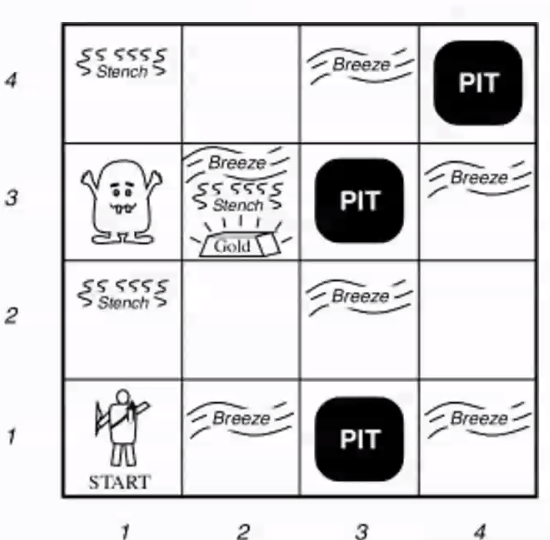
\includegraphics[scale=0.7]{wumpus.png}\\
	%TODO riscrivere
	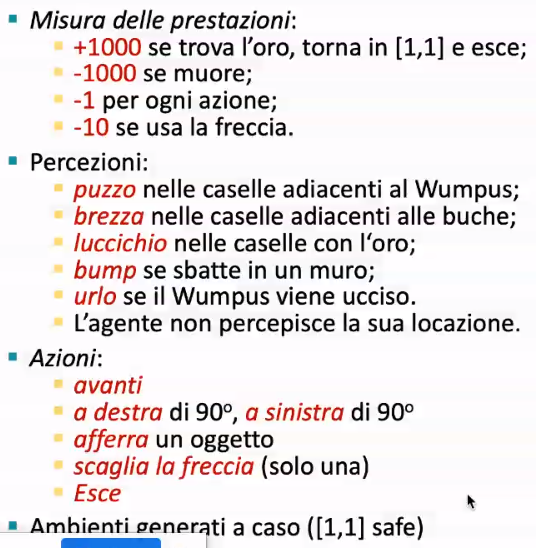
\includegraphics[scale=0.7]{wumpus2.png}
\end{center}
\paragraph{Uno scenario} \ldots
\paragraph{KB} Insieme di enunciati espressi in un linguaggio di rappresentazione.\\
L'agente interagisce con una KG con un'interfaccia funzionale \textbf{Tell-Ask}:
\begin{list}{}{}
	\item Tell
	\item Ask
	\item Retract
\end{list}
Enunciati in KG rappresentano conoscenza agente\ldots %TODO
\paragraph{Problema} Il problema da risolvere: data conoscenza KB che contiene\ldots vorrei sapere se un certo fatto $\alpha$ è vero di conseguenza, cioè se KB $soddisfa \alpha$
\paragraph{Programma di un agente KB} \ldots
Una  \textbf{base di conoscenza} è rappresentazione esplicita, parziale e compatta in linguaggio simbolico: contiene sia fatti espliciti (es. Pozzo in [3, 3]) ma anche fatti generali o regole (es: brezza in caselle adiacenti a pozzi)\\
Una base di dati invece solo base di dati e solo recupero.\\
La differenza è che la KB ha capacità inferenziale: derivare nuovi fatti da quelli memorizzati esplicitamente.
\paragraph{Trade-Off Fondamentale della Rappresentazione della Conoscenza} Trovare giusto compromesso tra linguaggio rappresentazione espressivo e la complessità del meccanismo inferenziale.\\
Pià linguaggio è espressivo meno è efficiente il meccanismo inferenziale. Obiettivi in contrasto, bisogna mediare e trovare \textbf{compromesso}.\\
\paragraph{Formalismi per la R.C.}
\begin{list}{}{}
	\item Sintassi
	\item Semantica
	\item Meccanismo inferenziale
\end{list}
\paragraph{Logica come linguaggio}
Qual è la complessità computazionale del problema KB $soddisfa \alpha$ nei vari linguaggi logici? Quali algoritmi decisione e strategia ottimizzazione?\\
Linguaggi logici: calcolo proposizionale (POP) e logica dei predicati (FOL). Sono adatti per la rappresentazione della conoscenza? Da una parte sono anche troppo complessi, in particolare il FOL. Dall'altra, ci sono meccanismi non posseduti da FOL e POP ma che sono utili nelle KB.\\
Rivistazione di PROP e FOL per rappresentazione conoscenza, con attenzione ad algoritmi e complessità. \textbf{Contrazioni}: linguaggi a regole e \textbf{programmazione logica}.
\section{Calcolo Proposizionale}
\paragraph{Sintassi} %TODO Sintassi calcolo proposizionale

\paragraph{Algoritmo TT-entails?}
\begin{list}{}{}
	\item KB $soddisfa \alpha$?
	\item Enumera tutte possibili interpretazioni KB ($k$ simboli, $2^k$ possibili interpretazioni)
	\item \ldots
\end{list}
\paragraph{Algoritmi per la soddisfacibilità (SAT)}
Usano KB come insieme di clasusole.
\paragraph{Algoritmo DPLL}
Parte da una KB in forma a clausole. Enumerazione in profondità di tutte le possibili interpretazioni alla ricerca di un modello. Tre miglioramenti rispetto TTEntails:
\begin{list}{}{}
	\item Terminazione anticipata
	\item Euristica dei simboli (o letterali) puri
	\item Euristica delle clausole unitarie
\end{list}
\paragraph{Simboli puri} Simbolo con stesso segno in tutte le clausole. Es \{A, notB\}, \{notB, notC\}, \{C, A\} A puro e B anche.\\
Nel determinare un simbolo se è puro possiamo trascurare occorrenze simbolo in clausole già rese vere. Se simbolo è puro può essere assegnato a T se positivo, F se negativo senza eliminare modelli.
\paragraph{Clausole unitarie}
%TODO
\end{document}
